\documentclass[11pt]{article}

% ---------------------------------------------------------------------------
% Preamble
% ---------------------------------------------------------------------------
\usepackage[T1]{fontenc}
\usepackage[utf8]{inputenc}
\usepackage{lmodern}
\usepackage[margin=1in]{geometry}
\usepackage{microtype}
\usepackage{amsmath,amssymb}
\usepackage{graphicx}
\usepackage{booktabs}
\usepackage{multirow}
\usepackage{xcolor}
\usepackage{enumitem}
\usepackage[font=small,labelfont=bf]{caption}
\usepackage[round,authoryear]{natbib}
\usepackage[colorlinks=true,linkcolor=blue!60!black,citecolor=blue!60!black,urlcolor=blue!60!black]{hyperref}
\usepackage[nameinlink,capitalize]{cleveref}

\graphicspath{{figures/pdf/}}

% Pending-result marker: every unfilled number in the draft is explicit.
\newcommand{\todo}[1]{\textcolor{red}{\textbf{[#1]}}}

\title{\textbf{Look Again: Self-Correcting Tool Use for\\ Panoramic Dental Radiograph Diagnosis}}

\author{%
  Reza Nadimi\thanks{Corresponding author. \todo{Affiliations and co-author list to be
  finalized.}}\\
  \todo{affiliations}
}
\date{October 2026}

% ---------------------------------------------------------------------------
\begin{document}
\maketitle

\begin{abstract}
Vision-language models (VLMs) applied zero-shot to panoramic dental radiographs fail
structurally: the best frontier models reach only 36--46\% exact-match accuracy against expert
labels, an 11B generalist falls below the majority-class floor, and calibration is poor
(ECE up to 0.68), because a single static forward pass cannot zoom into sub-patch pathology,
resolve the modality's left/right display convention, or verify an anatomical hypothesis before
committing to it. We present \textbf{VLM-DENTAL}, an agentic VLM trained on the DENTEX benchmark
around a different contract between the policy and its tools: \emph{grounding is a hypothesis to
interrogate, not an answer to trust}. Concretely, (1) the policy can correct its learned
grounding tool via \texttt{nudge\_crop}, a data-only tool taking box-relative fractional shifts
and rescales that a VLM can reason about linguistically; (2) a \emph{tiered perturbation}
mechanism makes this skill learnable from synthetic demonstrations --- the demonstrator
experiences deliberately imperfect tool output (45\% clean / 25\% small / 30\% large offsets,
decoupled from the detector's real error rate so demonstrations never go stale, and never
announced verbally so the skill survives to inference time); (3) the eight-tool interface
exposes continuous effect parameters (denoise strength, window center/width, contrast factor,
crop context), so tool calls carry \emph{how much}, not just \emph{which}; and (4) GRPO
reinforcement learning uses a ground-truth-anchored composite reward with multi-finding
set-matching whose efficiency term exempts locate-and-correct calls, so the reward never prices
out the behavior it teaches. A corpus-level analysis of 3{,}694 verified, decontaminated
synthetic traces shows the perturbation mechanism elicits a clean judgment gradient ---
corrective nudges on 38.4\% of large tool errors, 13.6\% of ambiguous ones, and 1.1\% of clean
outputs (ground-truth-anchored pathology locates), with recoveries up to IoU 0.07 $\to$ 0.94
--- demonstrating genuine visually-driven
self-correction rather than scripted steps. Evaluation uses DENTEX-native, leaderboard-comparable
set-matched metrics with paired bootstrap intervals and a frozen, leak-free protocol; end-to-end
training results are reported as runs complete. We position the work relative to concurrent
dental agentic systems and release the corpus, audit tooling, and all figure/table sources for
regenerability.
\end{abstract}

% ---------------------------------------------------------------------------
\section{Introduction}
\label{sec:intro}

Panoramic dental radiograph analysis requires assigning diagnostic findings to individual
teeth in standard FDI notation. General-purpose vision-language models (VLMs) offer a flexible
interface, but our zero-shot evaluation on DENTEX shows limited finding-level agreement with
expert annotations (\cref{sec:baselines}). The best reported pooled exact F1 is 0.222.
Image-level hit rates and calibration provide complementary evidence, but do not by themselves
identify the causes of these errors. Local detail, tooth identity, and orientation motivate an
agent that can inspect a region again before answering.

Medical and general-purpose tool-using systems provide relevant precedents
\citep{wu2026vtool,li2024mmedagent,zhang2025octotools,oralgptplus2026,oralagent2026}.
We focus on a specific failure point: a learned grounding model can return a plausible box for
the wrong region, and subsequent crops inherit that error. Rather than treating the box as an
authoritative observation, the policy should be able to inspect and revise it. Whether a
trained policy acquires this behavior, and whether it improves diagnosis, are empirical
questions addressed by the frozen evaluation design.

This paper develops and evaluates \sys{}, an agentic VLM for OPG diagnosis built around a
different contract between the policy and its tools: \emph{grounding is a hypothesis, not an
answer} (\cref{fig:concept}). \cref{fig:architecture,fig:training} give the complete system architecture (agent loop and offline
training stack), and \cref{fig:evidence,fig:traces} contrast the two trace arms on one image. Our contributions are:

\begin{figure}[tbp]
  \centering
  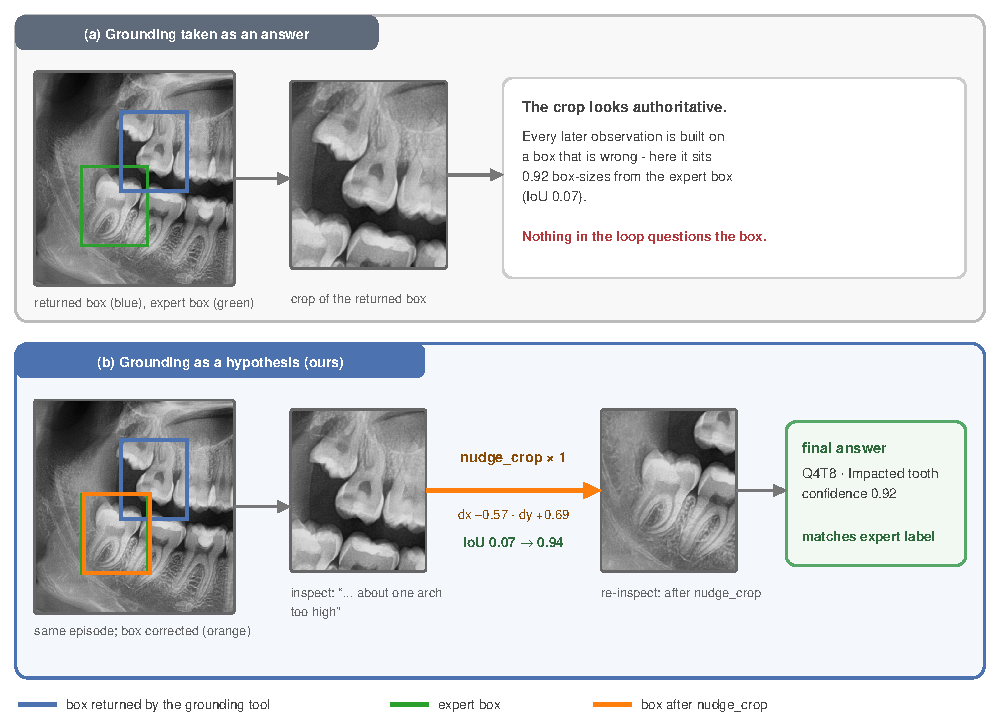
\includegraphics[width=\linewidth]{fig_concept}
  \caption{The central idea, on a real episode from the corpus (DENTEX image 127, an impacted FDI
  tooth 48). (a) When a grounding box is taken as an answer, the crop of that box looks
  authoritative and every later observation inherits its error --- here the returned box (blue)
  sits 0.92 box-sizes from the expert box (green; IoU 0.07). (b) \sys{} treats the box as a
  hypothesis: the policy sees a crop dominated by an upper molar, judges the box ``about one arch
  too high'', corrects it with one box-relative \texttt{nudge\_crop} (orange; IoU 0.94), and
  answers from the corrected view. Crops are native-resolution views of the box with 30\% padding, illustrative of what the zoom
  tool returns rather than the canonical-view geometry of \cref{fig:inputgeom}. Further episodes
  are in \cref{fig:gallery}; the full with-tools trace of another image is dissected in
  \cref{fig:evidence,fig:traces}.}
  \label{fig:concept}
\end{figure}

\begin{enumerate}[leftmargin=*,itemsep=2pt,topsep=3pt]
\item \textbf{A self-correcting grounding tool (\texttt{nudge\_crop}, \cref{sec:nudge}).}
The policy can shift and rescale a box it was \emph{already given} --- by the grounding model or
by a previous correction --- using box-relative fractional arguments (\texttt{dx\_frac},
\texttt{dy\_frac}, \texttt{scale}) that a VLM can reason about linguistically
(``shift right about half a tooth-width''), without re-running detection. We make box revision an explicit, inspectable action rather than an implicit change in the
policy's internal localization.
\item \textbf{A tiered perturbation mechanism that makes self-correction learnable
(\cref{sec:perturbation}).} Demonstrating correction behavior requires the demonstrator to
\emph{experience} tool error. During trace generation we return the expert-verified box for
annotated teeth (guaranteeing task solvability) but deliberately perturb the box
\emph{shown to the demonstrator} --- 45\% clean, 25\% small offsets (12--28\% of box size), 30\%
large offsets (45--75\%) --- with two design commitments: the rates are fixed constants decoupled
from the detector's real error rate, so demonstrations never go stale as the detector improves;
and errors are never announced verbally, so correction must be elicited by the returned image rather than an explicit error message.
Transfer of this behavior to the trained policy remains to be measured. A corpus-level analysis (\cref{sec:mechanism}) shows the mechanism elicits exactly the
intended behavior gradient in 3{,}694 generated demonstrations: corrective use of
\texttt{nudge\_crop} on 38.4\% of large offsets, 13.6\% of small ones (intermediate offsets),
and 1.1\% of clean boxes, on ground-truth-anchored pathology locates.
\item \textbf{A tool interface with continuous parameters (\cref{sec:tools}).} Tools expose
\emph{how much} effect to apply, not just which tool to call: \texttt{denoise(strength
$\in[0,1]$)}, \texttt{window\_level} with exact \texttt{center}/\texttt{width} values as an
override on top of presets, a multiplicative \texttt{enhance\_contrast} factor, and a tunable
\texttt{zoom\_crop} context margin. Tool calls therefore
carry real information beyond tool identity, and the policy can match processing intensity to
image characteristics.
\item \textbf{A ground-truth-anchored, correction-friendly reward (\cref{sec:reward}).} GRPO
training \citep{deepseek2025r1} uses a composite reward whose dominant term is a hard,
non-LLM-judge match against expert labels with multi-finding greedy one-to-one matching
(F1-style harmonic mean of recall and precision), and whose efficiency term scales a reference
budget with case complexity and \emph{exempts} \texttt{locate\_tooth} and \texttt{nudge\_crop}
from per-call cost --- so the reward never prices out the verification behavior it is trying to
teach, a failure mode we identified and removed by design.
\item \textbf{Label-anchored synthetic demonstrations and an audit trail
(\cref{sec:traces}).} 3{,}694 verified chain-of-thought tool-use traces over DENTEX and Tufts
(1{,}847 with tools, 1{,}847 single-turn without, exact 1:1 parity), generated by frontier models
under real tool execution in a LangGraph loop, verified cross-family, decontaminated of
directive leakage (105 traces regenerated; 0 leaks in the canonical corpus), and released as a
reusable resource. The verifier's rejection taxonomy (66 false-positive findings on healthy
scans, 15 ground-truth contradictions, 11 uncorrected spatial drifts) doubles as an audit of
what the perturbation mechanism does and does not elicit.
\end{enumerate}

We evaluate on DENTEX with its native structured metrics --- pooled, set-matched,
finding-level precision/recall/F1 with paired bootstrap intervals --- against zero-shot frontier
VLMs, the same backbone with and without tools, and a supervised specialist detector. The
training-side analyses in this draft are complete; the two-stage training runs (SFT, then GRPO)
are not yet reported, and their result cells are marked \todo{SFT/GRPO results pending first
hardware run} rather than extrapolated. Inference-time rules, skills, and serving optimizations are evaluated
separately on the training-derived dev split (\cref{sec:harness-serving}); they do not revise
the frozen primary protocol.

% ---------------------------------------------------------------------------
\section{Related Work}
\label{sec:related}

\paragraph{Supervised dental AI.}
The dominant paradigm in dental radiograph analysis is narrow, single-task supervised learning:
CNN and Faster R-CNN cephalometric landmark detectors, U-Net-style segmentation, FDI tooth-numbering
classifiers, and YOLO-family or Faster R-CNN detectors for caries, periapical lesions, and
impactions \citep{hamamci2024dentex}. The DENTEX benchmark consolidated this into a hierarchical
quadrant--enumeration--diagnosis task with expert-verified labels \citep{hamamci2024dentex} and
remains the most structured public benchmark for our problem. These supervised tasks differ from our episode-level setting, in which a policy can request
additional views and revise a grounding hypothesis. A systematic review of public dental imaging
datasets \citep{uribe2024systematic} screened 131{,}028 records and found only 16 datasets
meeting a minimal bar --- the data scarcity that motivates our synthetic-trace approach.

\paragraph{Reinforcement-learned reasoning in medical VLMs.}
Following the GRPO recipe \citep{deepseek2025r1}, \citet{hu2025medvlmr1} fine-tuned a 2B VLM with
GRPO on a few hundred examples and reported large gains over zero-shot across MRI, CT, and X-ray
VQA; Med-R1 extended this across eight modalities and found that lengthening the chain of thought
does not reliably improve accuracy --- reward alignment matters more than reasoning length
\citep{wang2025medr1}. HuatuoGPT-o1 \citep{chen2024huatuo} and OpenMedReason
\citep{openmedreason2026} build reasoning supervision by using a frontier model purely as a
\emph{verifier} of evidence-grounded traces. These reasoning-supervision approaches motivate our training recipe; our focus is the
additional interaction between a reasoning policy and revisable visual observations.

\paragraph{Agentic tool use in VLMs.}
MMedAgent trains an LLM to select among grounding, segmentation, and report tools
\citep{li2024mmedagent}; OctoTools generalizes the orchestration pattern \citep{zhang2025octotools}.
Closest in spirit is VTool-R1 \citep{wu2026vtool}, which trains a VLM with GRPO to call
Python-based visual-editing tools mid-reasoning, improving chart/table QA from 64.7\% to 71.7\%.
Its tools are generic image-editing primitives, its reward is a single outcome-accuracy term, and
its domain is not medical. Two concurrent dental systems must be addressed directly.
\textbf{OralGPT-Plus} \citep{oralgptplus2026} pairs trained CoT, two callable image tools
(zoom-in, contralateral mirror), and GRPO-style RL with a composite reward --- the closest
concurrent work, but it evaluates on its own benchmark with an LLM-judge-scored reward (whose
documented reward-hacking failure mode motivates our ground-truth-anchored accuracy term,
\cref{sec:reward}) and does not cleanly separate tool-use from RL effects.
\textbf{OralAgent} \citep{oralagent2026} is a broader prompted ReAct orchestrator around an
off-the-shelf model, not an RL-trained tool-use policy. Our emphasis is a box-relative corrective action and a controlled evaluation of tools and RL,
rather than a claim to originate dental agents or medical tool use. Comparisons should account
for differences in datasets, available supervision, and scoring protocols.

\paragraph{Procedural context and speculative serving.}
The rules-and-skills extension follows the inspectable \texttt{SKILL.md} convention with
progressive disclosure \citep{agentskills2026}. Its contribution here is a provenance-tracked
integration with the shared dental dispatcher, not a new knowledge-file format.
Speculative decoding uses a draft proposal and target verification to accelerate generation
\citep{leviathan2023fast,chen2023accelerating}; vLLM provides the serving substrate
\citep{kwon2023efficient}. We treat serving speed and clinical-task performance as separate
measurements, and test output equivalence on the actual multimodal episodes rather than
assuming it from the algorithm alone.

\paragraph{Label-anchored synthetic reasoning traces.}
Frontier LLMs can generate and verify reasoning-trace training data of sufficient quality for
downstream fine-tuning \citep{chen2024huatuo,openmedreason2026}, replacing prospective expert
annotation with expert-\emph{verified benchmark labels} plus cross-model automated checks. We
extend this pattern to \emph{multi-turn tool-use} traces: the demonstrator operates a real tool
suite under real tool feedback (including deliberately imperfect tool output, \cref{sec:perturbation}),
and an independent cross-family verifier audits every trace against expert labels before it
enters the training set.

% ---------------------------------------------------------------------------
\section{\sys{}: System and Method}
\label{sec:method}

\subsection{Problem setup and agent loop}
\label{sec:setup}

An OPG $I$ is annotated as a \emph{set} of findings $F = \{f_1, \dots, f_m\}$ (possibly empty for
a healthy image), where each finding $f = (\text{quadrant}, \text{tooth position},
\text{diagnosis})$ uses FDI two-digit notation over DENTEX's four diagnosis classes
(caries, deep caries, periapical lesion, impacted tooth). The agent receives the image and a
registry of tools, and produces a sequence of turns; each turn contains free-form clinical
reasoning and zero or more structured tool calls, and the loop ends with a structured final
answer reporting \emph{every} finding the agent commits to. The same agent loop is used for
synthetic data generation, RL rollouts, and evaluation, and tool calls execute for real against
the source image at every stage (\cref{fig:pipeline}); a single shared dispatcher defines which
tools consume the image and which image they operate on, so the training and inference
environments cannot drift apart. Tool calls are capped at 50 per episode, counted by calls
rather than turns, and parsed by a bracket-counting JSON extractor that repairs truncated or
markdown-wrapped outputs.

\begin{figure}[tbp]
  \centering
  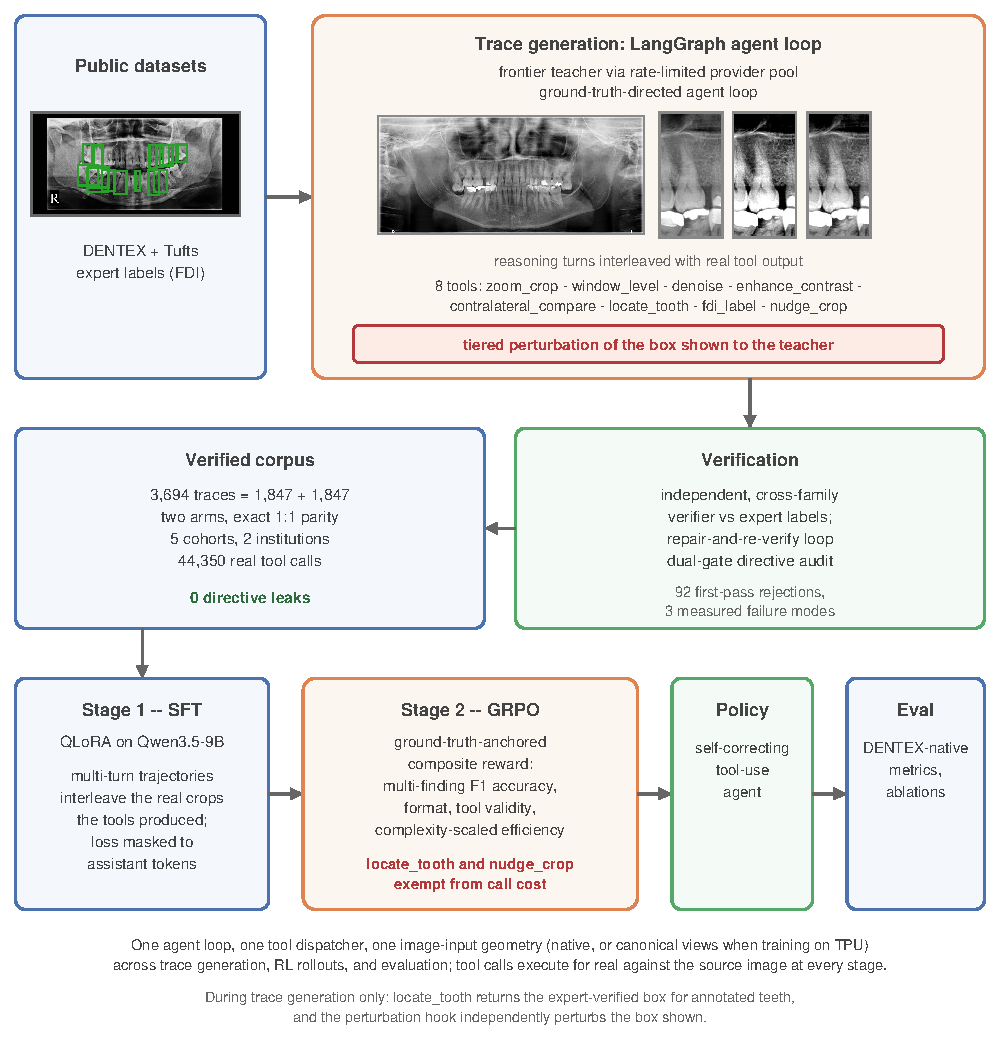
\includegraphics[width=\linewidth]{fig_pipeline}
  \caption{The \sys{} pipeline. Traces are synthesized by a frontier teacher operating a real
  tool suite in a LangGraph loop (with the tiered perturbation hook of \cref{sec:perturbation}),
  verified cross-family against expert labels, and used for SFT followed by GRPO with a
  ground-truth-anchored composite reward. Tool calls execute for real against the source image
  at every stage; the radiograph and crop pixels are real assets from the corpus (the image
  whose trace anatomy is dissected in \cref{fig:traces}).}
  \label{fig:pipeline}
\end{figure}

\subsection{System architecture}
\label{sec:architecture}

\cref{fig:architecture} shows the complete system. Five component groups surround one agent
core --- a Qwen3.5-9B vision-language policy running the loop of \cref{sec:setup}: a data layer
(\cref{fig:datasets}: registry-driven loaders for the two in-use sources, DENTEX and Tufts; a
candidate pool of eight further public panoramic datasets, promoted only after their annotation
semantics are verified; and surgical per-image Hugging Face caching), the trace
synthesis stack of \cref{sec:traces}, the two training stages of \cref{sec:reward}, and an
evaluation layer (\cref{sec:eval}) whose probes feed model selection on a fixed dev split.

\begin{figure}[tbp]
  \centering
  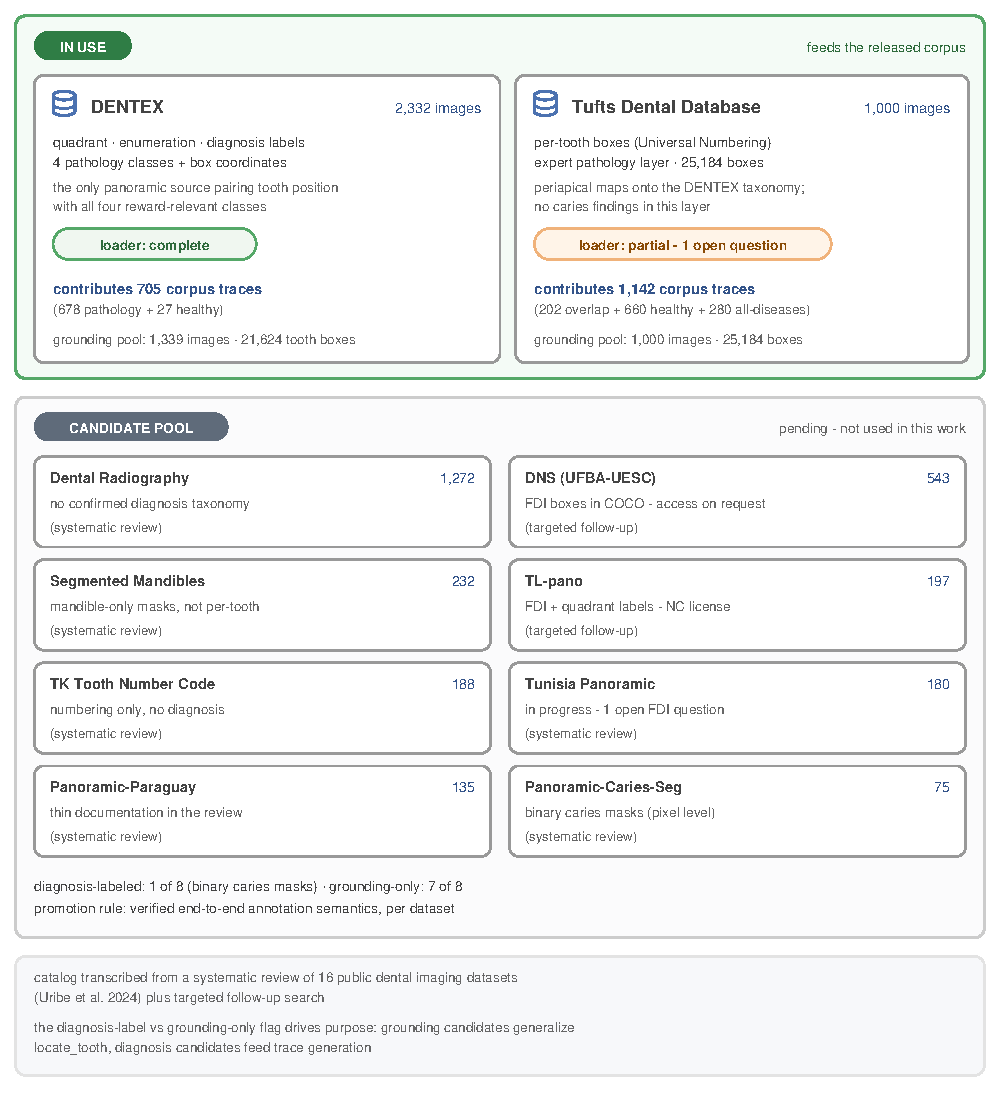
\includegraphics[width=\linewidth]{fig_datasets}
  \caption{The data layer. Two sources are in use --- DENTEX (the only panoramic dataset
  pairing tooth position with all four reward-relevant pathology classes) and the Tufts Dental
  Database (per-tooth boxes plus an expert pathology layer whose periapical class maps onto the
  DENTEX taxonomy). Eight further public panoramic datasets are catalogued as candidates and
  deliberately \emph{not} used: each would be promoted only after its annotation semantics are
  verified end-to-end, and two loaders currently stop at exactly one open question rather than
  guess. The diagnosis-label vs grounding-only flag drives purpose: grounding candidates
  generalize \texttt{locate\_tooth}, diagnosis candidates would feed trace generation.}
  \label{fig:datasets}
\end{figure}

\begin{figure}[tbp]
  \centering
  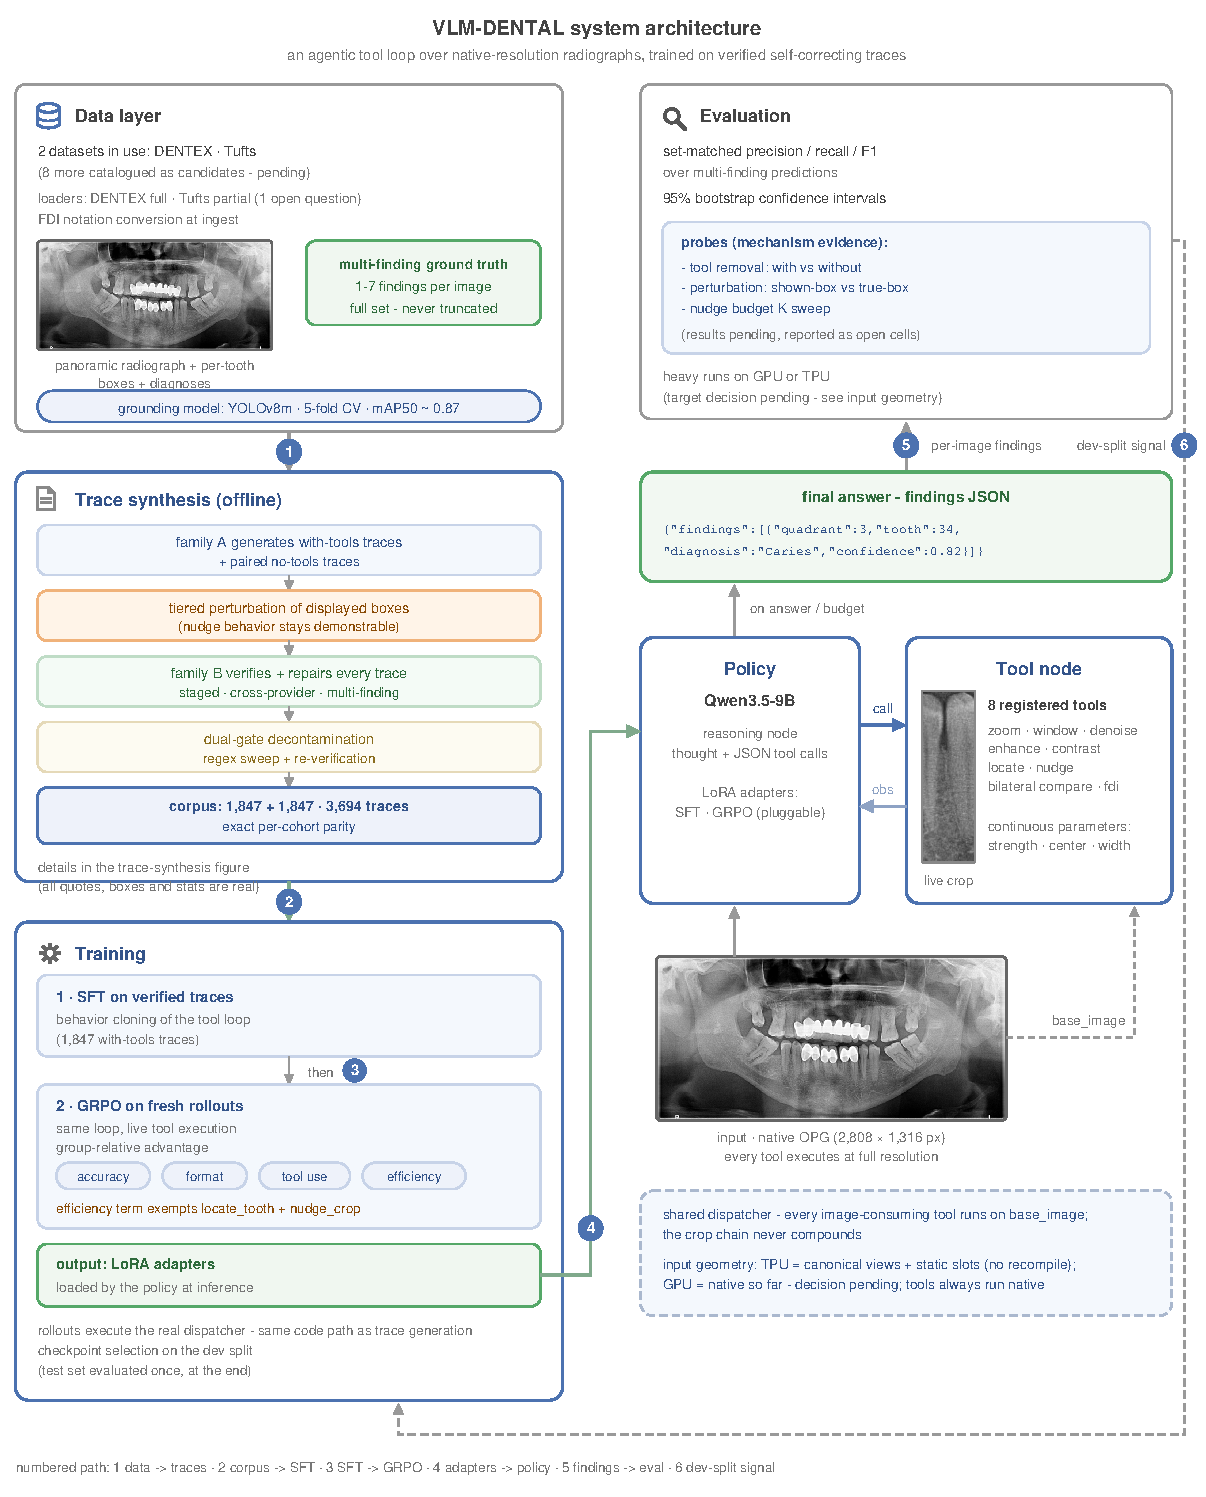
\includegraphics[width=\linewidth]{fig_architecture}
  \caption{The \sys{} architecture. One agent loop, one shared tool dispatcher, and one
  canonical vision geometry are shared by trace generation, RL rollouts, and evaluation; the
  trace synthesis stack produces the verified corpus consumed by SFT and GRPO; evaluation
  probes select on a dev split only, with the test split run once at the end. Numbered badges
  trace the corpus-to-policy life cycle (legend in the figure); radiograph and crop pixels are
  real assets from the corpus.}
  \label{fig:architecture}
\end{figure}

Three single-source-of-truth decisions hold the system together. First, one shared dispatcher
defines, for every tool, whether and \emph{which} image it consumes --- always the native source
image --- so the trace-generation loop, the GRPO rollout loop, and the evaluation runner cannot
silently diverge; the dispatcher exists precisely because the two loops originally duplicated
this logic and the rollout side drifted onto a compounding image state, a real bug that silently
invalidated rollouts. Second, the image-input geometry lives in one module and is an explicit
flag, not an implicit behavior (\cref{fig:inputgeom}). The two candidate execution targets make
different demands: TPU training requires aspect-preserving canonical views with static
vision-slot padding so XLA compiles a single graph and never recompiles, while GPU runs so far
feed original images with dynamic shapes; which target the project settles on --- a GPU
(RTX 4090 / RTX Pro 6000 / A100) or a TPU v5e-8 cluster --- is deliberately deferred to the
first GPU run. Whichever is chosen applies identically across SFT, RL, and evaluation, and in
both modes every tool operates on native-resolution pixels, so coordinates the model was trained
to emit remain valid at inference. Third, the conversion from DENTEX's zero-indexed annotation rows
to FDI notation has exactly one implementation, called by the reward, the verifier, and the
metrics alike --- an indexing bug cannot recur independently in several subsystems.

\begin{figure}[tbp]
  \centering
  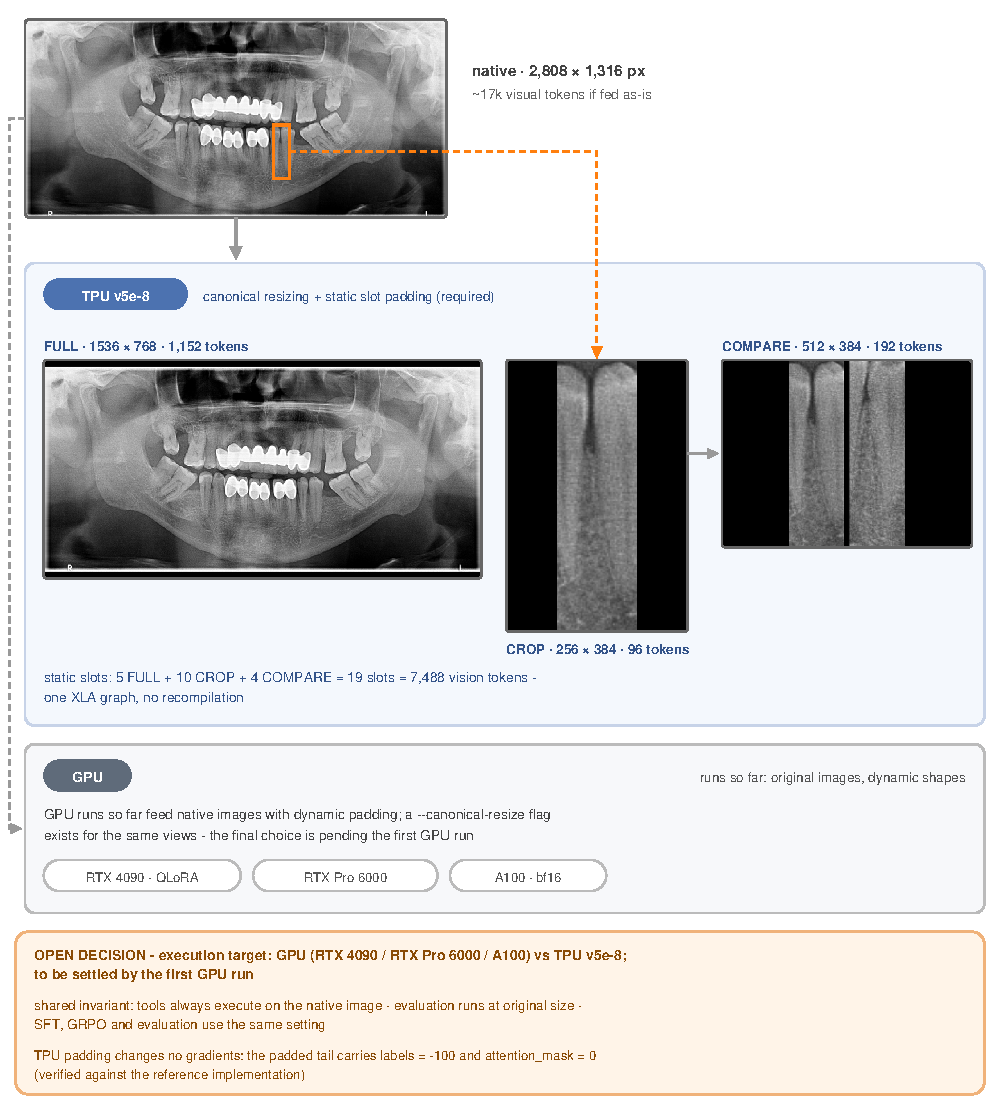
\includegraphics[width=\linewidth]{fig_input_geometry}
  \caption{Image-input geometry: two execution targets, one invariant. \textbf{TPU:} the policy
  sees aspect-preserving canonical views in three fixed families (renders produced by the
  geometry module itself, and the \texttt{contralateral\_compare} tool, from a DENTEX image),
  padded to a static 19-slot budget of 7{,}488 vision tokens so XLA compiles one graph; the
  padded tail carries $\text{labels}=-100$ and $\text{attention\_mask}=0$, so padding changes no
  gradient. \textbf{GPU:} runs so far feed original images with dynamic shapes. The choice
  between the targets is explicitly open pending the first GPU run; in both, tools always
  execute on the native image and evaluation runs at original size.}
  \label{fig:inputgeom}
\end{figure}

\subsection{A tool suite with continuous parameters}
\label{sec:tools}

The registry exposes eight tools (\cref{tab:tools}). The deliberate design choice throughout is
that tools expose \emph{how much} effect to apply as a continuous or overridable parameter, not
just a fixed on/off call: denoising takes a continuous \texttt{strength}, windowing takes exact
\texttt{center}/\texttt{width} values as an override on top of tissue presets, contrast takes a
multiplicative \texttt{factor}, and cropping takes a tunable context margin. A policy calling
\texttt{denoise(strength=0.3)} versus \texttt{denoise(strength=0.9)} is expressing a
patient-specific judgment about how grainy a crop is --- information a fixed three-level menu
cannot carry --- and the resulting tool-call stream is correspondingly more informative to train
on and to audit.

\begin{table}[tbp]
  \centering
  \small
  \caption{The \sys{} tool suite. Continuous or overridable parameters are shown in
  \emph{italics}; data-only tools return coordinates rather than images.}
  \label{tab:tools}
  \begin{tabular}{llp{6.4cm}}
    \toprule
    Tool & Key parameters & Purpose \\
    \midrule
    \texttt{zoom\_crop} & bbox, \emph{padding\_frac} & High-resolution crop of a region with a tunable context margin \\
    \texttt{window\_level} & preset; \emph{center}, \emph{width} & Radiological intensity windowing (bone/enamel/soft-tissue), exactly overridable \\
    \texttt{denoise} & method, \emph{strength} $\in[0,1]$ & Edge-preserving bilateral or median filtering matched to crop noise \\
    \texttt{enhance\_contrast} & \emph{factor} & Multiplicative contrast adjustment for subtle lesions \\
    \texttt{contralateral\_compare} & bbox, quadrant & Side-by-side mirror crop, constrained to the correct jaw half, for bilateral symmetry assessment \\
    \texttt{locate\_tooth} & FDI tooth & YOLOv8m grounding (32 classes, one per FDI position); returns a box \\
    \texttt{fdi\_label} & quadrant, position & FDI notation conversion and validation \\
    \texttt{nudge\_crop} & bbox, \emph{dx\_frac}, \emph{dy\_frac}, \emph{scale} & Correct a box the agent was already given, without re-running detection \\
    \bottomrule
  \end{tabular}
\end{table}

\subsection{Self-correcting grounding: \texttt{nudge\_crop}}
\label{sec:nudge}

The grounding tool is a YOLOv8m detector fine-tuned on 2{,}339 DENTEX+Tufts images with 46{,}808
tooth boxes, trained with 5-fold cross-validation (one class per FDI quadrant--position pair)
(\cref{fig:groundingcv}; full per-fold numbers in \cref{app:grounding}).
It is strong --- held-out \emph{target} mAP50 of 0.93--0.96 with precision up to 0.986 on
annotated teeth --- but it is a 32-class detector operating under per-fold variance, and its
errors are exactly the kind that poison downstream reasoning: a box shifted by half a
tooth-width produces a crop that still \emph{looks} like a plausible anatomical region while
showing the wrong tooth.

\begin{figure}[tbp]
  \centering
  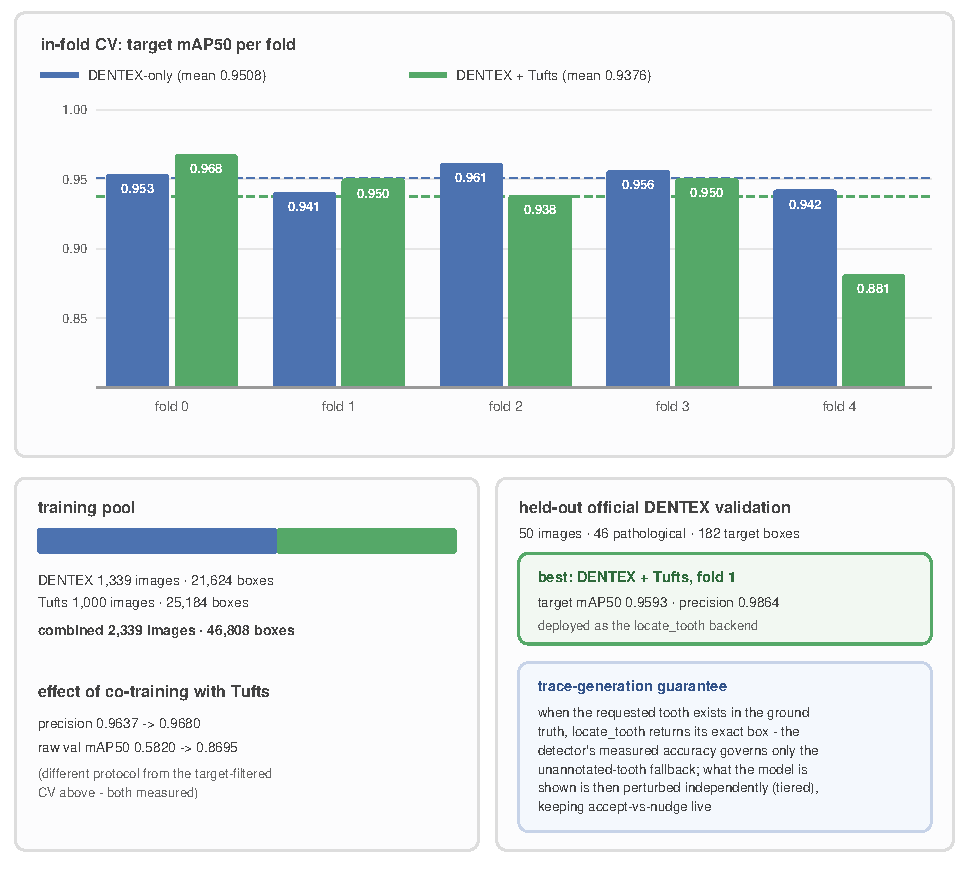
\includegraphics[width=\linewidth]{fig_grounding_cv}
  \caption{The \texttt{locate\_tooth} backend: YOLOv8m trained with 5-fold cross-validation on
  the combined DENTEX+Tufts pool (2{,}339 images, 46{,}808 tooth boxes). Left: in-fold
  target mAP50 per fold for the DENTEX-only and multi-dataset models (means 0.9508 / 0.9376).
  Right: pool composition, the held-out official DENTEX validation (best target mAP50 0.9593 at
  precision 0.9864 --- the deployed checkpoint), and the trace-generation guarantee: when a
  requested tooth exists in the ground truth, \texttt{locate\_tooth} returns its exact box, and
  only the \emph{displayed} copy is perturbed. Exact per-fold numbers in \cref{app:grounding}.}
  \label{fig:groundingcv}
\end{figure}

\texttt{nudge\_crop} turns that failure mode into an interaction. It takes a box the policy was
\emph{already given} (by \texttt{locate\_tooth} or a previous \texttt{nudge\_crop} --- never
asserted from nowhere) and returns adjusted coordinates: a shift $(\texttt{dx\_frac},
\texttt{dy\_frac})$ expressed as fractions of the box's own width and height, and a rescale
\texttt{scale} around the new center, clamped to image bounds. The tool is deliberately
\emph{data-only}: it computes coordinates, and the policy must pair it with \texttt{zoom\_crop}
to actually see the corrected region. Two consequences follow. First, the fractional,
box-relative parameterization is what a VLM can reason about reliably --- ``shift left by about
half the box'' --- rather than raw pixel coordinates at an arbitrary zoom level. Second, because
each correction must be followed by a verification crop, the loop enforces an
inspect--correct--re-inspect cycle rather than a single blind adjustment. This is the mechanism
neither concurrent dental agentic system provides: their tools are fixed operations whose
outputs the policy can only accept.

\subsection{Tiered perturbation: making self-correction learnable}
\label{sec:perturbation}

A policy can only learn to interrogate its tools if its teachers did. The core difficulty is
that an idealized demonstrator --- one whose grounding tool always returns the right box ---
demonstrates \emph{trusting} the tool, and SFT on such traces teaches exactly the wrong
reflex. At the same time, blind exploration by the demonstrator would collapse the yield of
usable traces.

Our resolution (\cref{fig:mechanism}) separates what the grounding tool \emph{computes} from
what the demonstrator \emph{sees}. During trace generation, \texttt{locate\_tooth} operates in a
ground-truth-grounding mode: for an annotated tooth it returns the expert-verified box
(guaranteeing the demonstration remains solvable), while for exploratory calls on unannotated
teeth it falls back to real detector inference. Then, independently of how the box was obtained,
a \emph{perturbation roll} decides what is displayed:

\begin{itemize}[leftmargin=*,itemsep=1pt,topsep=2pt]
  \item \textbf{none} (45\%): the box is shown as computed --- a clean accept-and-proceed demonstration;
  \item \textbf{small} (25\%): a synthetic offset of 12--28\% of the box's own size per axis,
  random sign --- a genuine judgment call that the zoom margin often absorbs, and that the prompt
  deliberately does \emph{not} resolve either way;
  \item \textbf{big} (30\%): an offset of 45--75\% per axis --- sized to be visually self-evident.
\end{itemize}

Offsets are applied with \texttt{nudge\_crop}'s own shift-and-clamp math, so every perturbed box
is one the correction tool could plausibly have produced or fixed; the unperturbed box is logged
internally for auditing but never shown. Two design commitments matter more than the numbers:

\paragraph{Fixed rates, decoupled from detector accuracy.}
The perturbation probabilities are configured constants, not a reflection of the grounding
model's measured error rate. This is a deliberate decoupling: if ``how often the model must
verify'' tracked the detector's live precision, then every improvement to the detector would
silently reduce the frequency of demonstrated correction, and traces generated under the old
detector would teach a stale behavior. With fixed rates, today's corpus remains valid as the
grounding tool improves --- a property this project exercised for real, as the detector's
validated mAP50 improved from 0.58 (DENTEX-only) to 0.87--0.96 (multi-dataset) while the trace
corpus stayed in use unchanged.

\paragraph{No verbal cue; magnitude carries the signal.}
Nothing in the trace-generation prompt marks a perturbed box as wrong. A verbal cue (``this box
needs correction'') would exist only during data generation and not at RL or inference time, so
teaching the model to respond to it would be a shortcut that fails exactly when it matters. The
big tier is therefore sized to be self-evident from the crop alone, and the small tier is left
genuinely ambiguous --- the demonstrator has to look and judge, which is precisely the skill the
deployed policy must exercise with no ground truth available at all.

\begin{figure}[tbp]
  \centering
  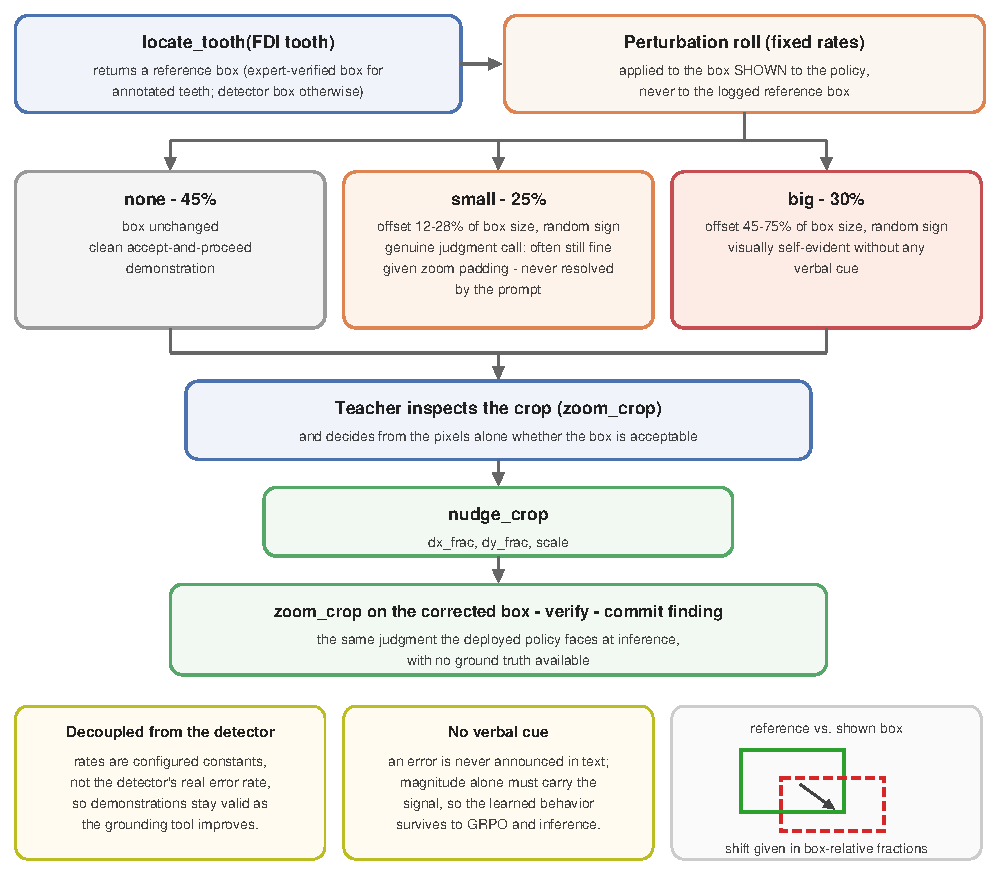
\includegraphics[width=\linewidth]{fig_perturbation_mechanism}
  \caption{The tiered perturbation mechanism and the correction loop it trains. The perturbation
  applies to the box shown to the policy only; offsets reuse \texttt{nudge\_crop}'s own math; and
  no verbal cue marks an error, so the offset magnitude alone must carry the signal.}
  \label{fig:mechanism}
\end{figure}

\subsection{Trace generation, verification, and decontamination}
\label{sec:traces}

Traces are generated by a frontier teacher (Gemini 3.5 Flash Lite or MiniMax M3, routed through
a rate-limited provider pool) that is directed toward the expert labels for the image but writes
its own reasoning and tool calls turn by turn under real tool feedback. Generation is
ground-truth-directed by design: blind exploration by an untuned model would tank the yield of
correctly-labeled demonstrations. Every trace then passes an independent, cross-family
\emph{verifier} conditioned on the image and the expert labels, which rejects reasoning not
supported by what the model was actually shown. Verification is staged rather than monolithic
(\cref{fig:multistage}): a strict pass checks diagnostic correctness, FDI validity, and whether
every claim is supported by what the model was actually shown --- treating valid
\texttt{nudge\_crop} correction loops as evidence of diligence rather than as errors --- and
rejected traces are routed to a verifier-editor that surgically repairs FDI labels, diagnosis
labels, and formatting while preserving the clinical chain of thought; the repaired trace is
re-verified before promotion. Both stages are cross-family by construction: the generator and
the verifier are routed through separate provider pools spanning different model families
(Gemini, MiniMax, NVIDIA NIM, Groq, OpenRouter), so a generator's blind spot is unlikely to be
shared by its judge. Because generation is conditioned on privileged information, traces are
scanned for \emph{directive leakage} --- the demonstrator echoing its hidden instructions in its
reasoning --- and leaking cases are excised and regenerated under a dual gate (zero-leak regex
audit + verifier re-approval); the canonical corpus contains zero leaks.

\begin{figure}[tbp]
  \centering
  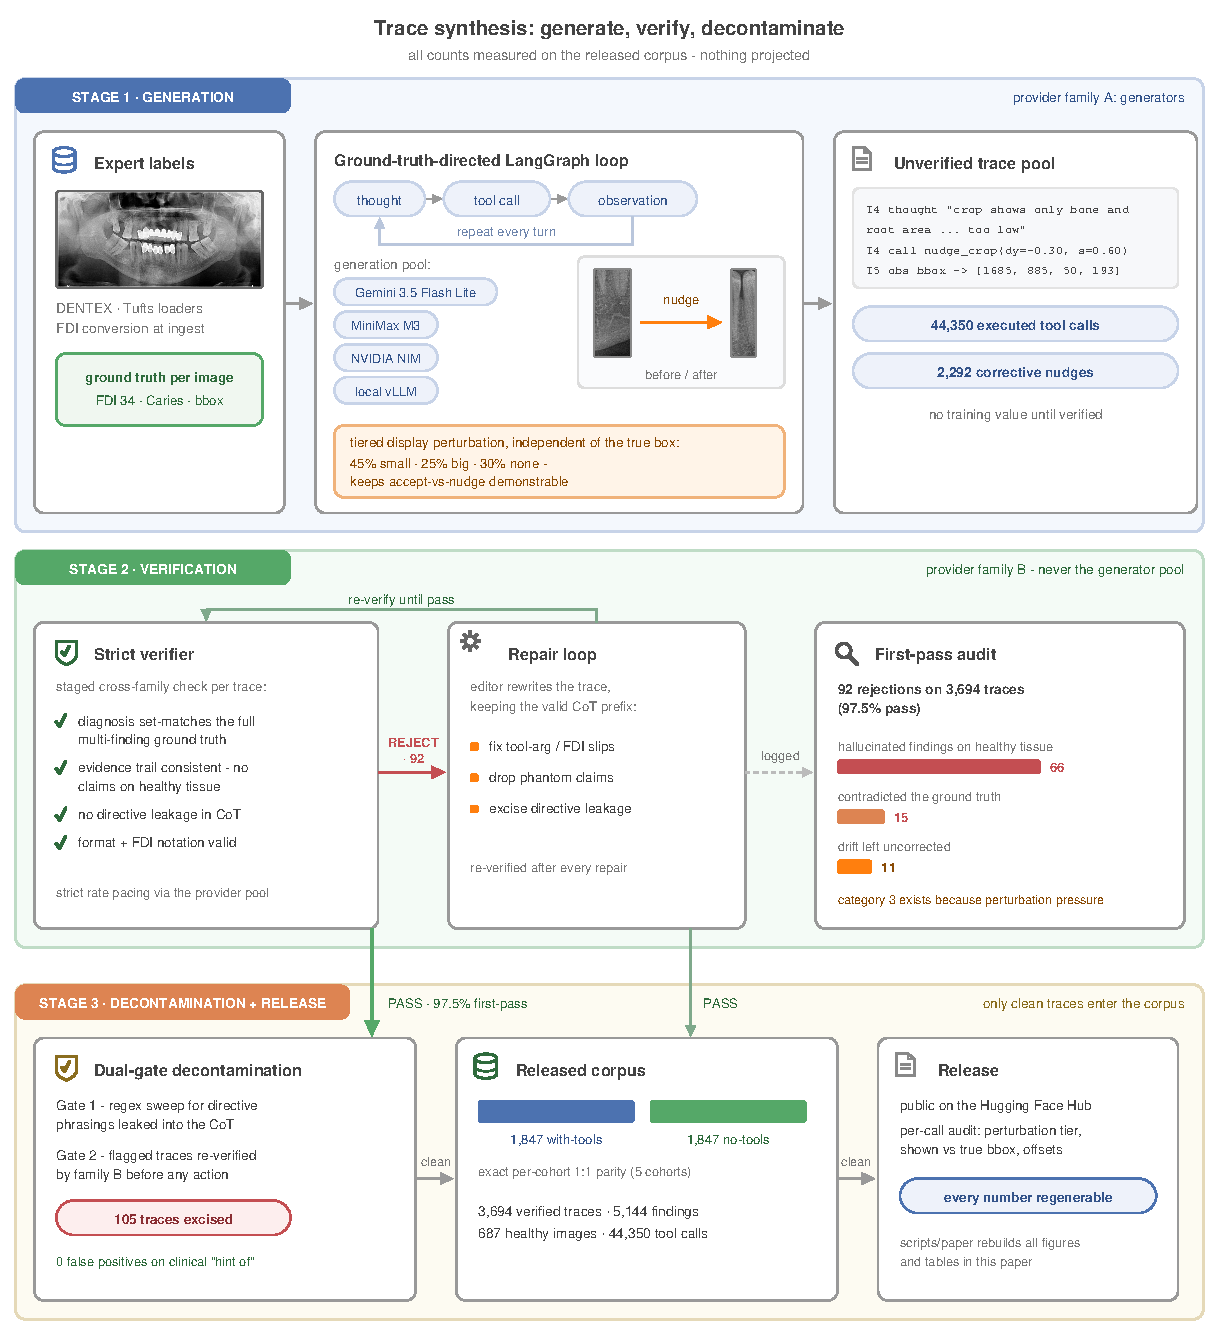
\includegraphics[width=0.92\linewidth]{fig_trace_multistage}
  \caption{Multi-stage trace synthesis. Generation (provider family A) runs a
  ground-truth-directed LangGraph loop with real tool execution and the tiered perturbation
  hook; staged verification (deliberately a \emph{different} provider family) combines a strict
  clinical pass with a repair-and-re-verify loop; a dual-gate leak audit and corpus assembly
  produce the frozen canonical release; the audit bars are measured counts. The verifier's
  92 first-pass rejections span three
  categories --- the third (uncorrected spatial drift) exists only because the perturbation
  mechanism creates genuine judgment pressure.}
  \label{fig:multistage}
\end{figure}

\begin{figure}[tbp]
  \centering
  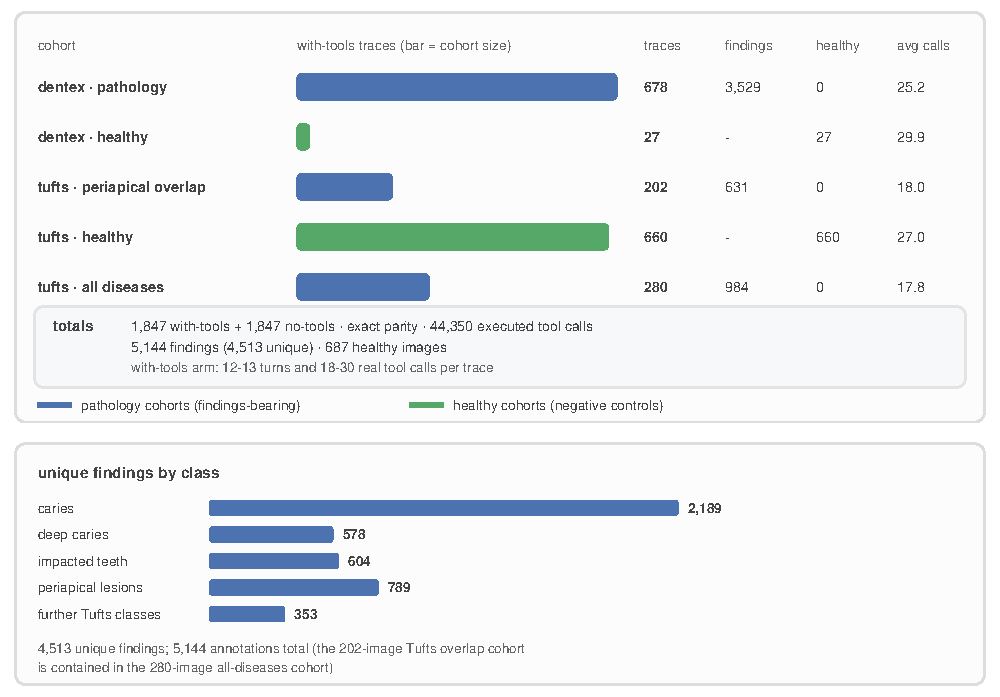
\includegraphics[width=\linewidth]{fig_corpus_composition}
  \caption{Corpus composition (measured from the released trace files). Five cohorts --- three
  findings-bearing, two healthy negative controls --- exist in two exact arms (with-tools and
  no-tools) with per-cohort 1:1 parity; the with-tools corpus carries 5{,}144 finding-level
  annotations (4{,}513 unique: the 202-image Tufts overlap cohort is contained in the 280-image
  Tufts all-diseases cohort, so its findings are counted in both). Class mix of the unique
  findings below; the teacher surveys every finding on an image, and healthy scans carry empty
  finding sets.}
  \label{fig:corpus}
\end{figure}

The resulting corpus (\cref{tab:corpus}, \cref{fig:corpus}) comprises 3{,}694 verified traces over 1{,}847 images
from two institutions: 1{,}847 interactive with-tools traces and 1{,}847 single-turn no-tools
traces in exact 1:1 parity --- the paired design that lets the evaluation isolate the
contribution of the tools (\cref{sec:eval}). The with-tools corpus carries 5{,}144
finding-level ground-truth annotations across cohorts (4{,}513 unique: the 202-image Tufts
overlap cohort is contained in the 280-image Tufts all-diseases cohort, so its 631 findings are
counted twice), spanning caries (2{,}189), deep caries (578), impacted teeth (604), periapical
lesions (789 unique), and three further Tufts lesion classes (353); multi-finding images carry
up to 23 annotated findings, and the teacher surveys every finding on the image. Healthy scans
are included as negative controls with empty finding sets. The verifier rejected 92 traces
across three failure modes: 66 hallucinated findings on healthy scans, 15 ground-truth
contradictions (wrong diagnosis class or swapped quadrants), and 11 uncorrected spatial drifts
--- cases where the teacher diagnosed from a visibly displaced box without issuing a corrective
\texttt{nudge\_crop}. The third category is direct evidence that the perturbation mechanism
creates real, auditable judgment pressure rather than a scripted step. Across the with-tools
corpus the teacher averaged 12--13 turns and 18--30 real tool calls per trace
(\cref{tab:corpus}); the full call distribution is shown in \cref{fig:toolusage}.

\begin{table}[tbp]
  \centering
  \small
  \caption{The verified corpus, regenerated from the released trace files. With-tools and
  no-tools cohorts are in exact 1:1 parity (checkmarks). Turns and tool calls are for the
  with-tools side; findings are counted per cohort (the Tufts overlap cohort is a subset of the
  Tufts all-diseases cohort, so its findings are counted in both).}
  \label{tab:corpus}
  \begin{tabular}{lrrrrrr}
\toprule
Cohort & With-tools & No-tools & Findings & Healthy & Turns & Tool calls \\
\midrule
DENTEX pathology & 678 & 678~\checkmark & 3529 & 0 & 12.9 & 25.2 \\
DENTEX healthy (negative controls) & 27 & 27~\checkmark & 0 & 27 & 13.4 & 29.9 \\
Tufts overlap pathology & 202 & 202~\checkmark & 631 & 0 & 12.0 & 18.0 \\
Tufts healthy (negative controls) & 660 & 660~\checkmark & 0 & 660 & 12.8 & 27.0 \\
Tufts 4-disease pathology & 280 & 280~\checkmark & 984 & 0 & 11.7 & 17.8 \\
\midrule
Total & 1847 & 1847~\checkmark & 5144 & 687 & -- & -- \\
\bottomrule
\end{tabular}
\end{table}

\begin{figure}[tbp]
  \centering
  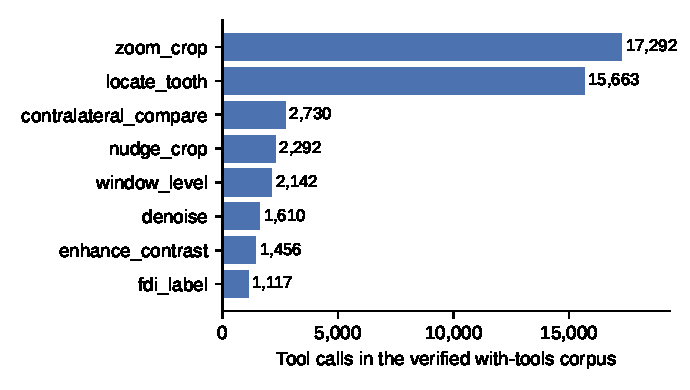
\includegraphics[width=0.62\linewidth]{fig_tool_usage}
  \caption{Recorded tool-call attempts over the verified with-tools corpus (44{,}350 across
  1{,}847 traces, of which 48 were invalid --- e.g.\ a hallucinated \texttt{localize\_tooth} ---
  and returned a standard error observation to the agent).
  \texttt{zoom\_crop} and \texttt{locate\_tooth} dominate;
  \texttt{nudge\_crop} appears 2{,}292 times as genuine mid-episode correction.}
  \label{fig:toolusage}
\end{figure}

\subsection{Anatomy of a trace: with tools vs.\ without}
\label{sec:traceanatomy}

\cref{fig:traces} shows both halves of the paired corpus for one DENTEX image (a carious FDI
tooth 34, a single finding). The no-tools trace is one turn: a fluent, well-structured direct
diagnosis that happens to reach the right answer, with no evidence trail --- the reasoning
cannot be checked against anything the model was actually shown, and the model never had the
opportunity to be wrong and recover. The with-tools trace for the same image runs 23 turns and
22 real tool calls and demonstrates the full behavioral repertoire the perturbation mechanism is
designed to elicit: the grounding box for tooth 34 was inspected, judged wrong (``the crop shows
only bone/root area \ldots the box appears to be too low''), and corrected three times with
box-relative \texttt{nudge\_crop} shifts until re-inspection confirmed the crown; a
contralateral symmetry comparison and a contrast-enhanced re-inspection followed before the
structured final answer, which matches the expert label.

\begin{figure}[tbp]
  \centering
  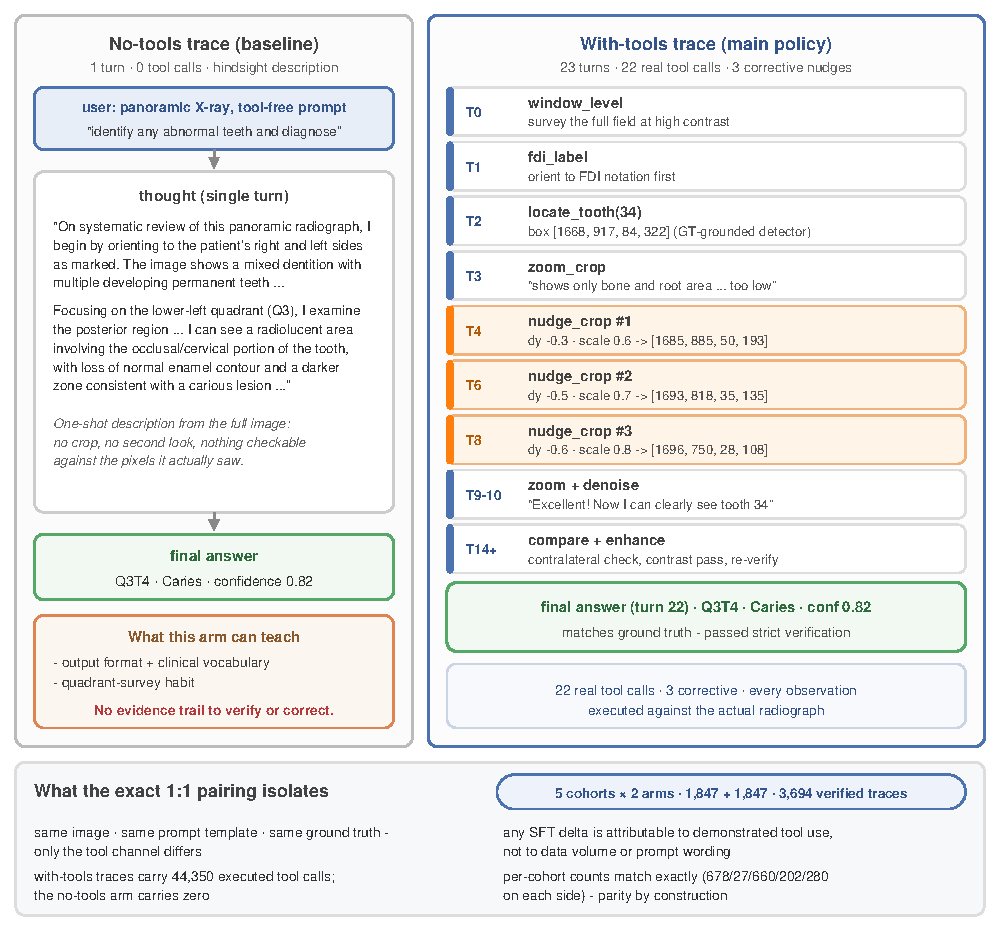
\includegraphics[width=0.88\linewidth]{fig_traces_comparison}
  \caption{Two training traces for the same image (DENTEX, carious FDI 34) and the same expert
  label. Left: the real radiograph with the with-tools evidence trail --- the returned grounding
  box (blue), the three corrective \texttt{nudge\_crop} boxes (orange, light to dark, magnified
  in the inset; the arrow marks the upward walk from the returned box to the corrected one),
  and the expert box (green dashed); all coordinates are the
  values actually returned by the tools, and the right panel shows the crop the teacher finally
  saw. Middle: the single-turn no-tools trace --- fluent, correct, and unverifiable. Right: the
  with-tools trace (23 turns, 22 real tool calls), in which the grounding box is inspected,
  judged wrong, corrected three times, and re-inspected before the answer; quotes are abridged
  from the released traces. The two arms exist in exact per-cohort 1:1 parity, so the evaluation
  can vary only the tool interface.}
  \label{fig:traces}
\end{figure}

The paired design is what makes this contrast usable rather than anecdotal. With 1{,}847
with-tools and 1{,}847 no-tools traces in exact per-cohort parity, the evaluation can hold the
image and the label fixed and vary only the tool interface, isolating what interactive tool use
adds over single-pass reasoning (\cref{sec:eval}). The no-tools traces are retained
deliberately: they teach output format and clinical vocabulary and provide the baseline arm of
every comparison --- but they are documented as ground-truth-directed single-pass generation
(closer to hindsight rationalization than blind discovery), a tradeoff \cref{sec:traces} made
explicit rather than hidden.

\subsection{Training: SFT then GRPO with a correction-friendly reward}
\label{sec:reward}

Stage 1 (SFT) fine-tunes Qwen3.5-9B \citep{bai2025qwen25vl} with QLoRA \citep{dettmers2023qlora}
on the verified with-tools traces, teaching the \emph{shape} of the behavior: well-formed
reasoning, well-formed tool calls with continuous parameters, and structured multi-finding final
answers. Multi-turn trajectories interleave the real crops the tools produced, and loss is
masked to assistant tokens only.

Stage 2 (GRPO \citep{deepseek2025r1}) optimizes the composite reward
\[
  R = w_{\text{acc}} R_{\text{acc}} + w_{\text{fmt}} R_{\text{fmt}}
    + w_{\text{tool}} R_{\text{tool}} + w_{\text{eff}} R_{\text{eff}},
\]
with three properties that matter for this task:

\paragraph{Ground-truth-anchored, multi-finding accuracy.}
$R_{\text{acc}}$ is a hard, non-LLM-judge match against expert labels. Predicted findings are
matched to annotated findings one-to-one by greedy highest-score-first assignment; each matched
pair scores $0.25 \cdot
\mathbf{1}[\text{quadrant}] + 0.25 \cdot \mathbf{1}[\text{position}] + 0.50 \cdot
\mathbf{1}[\text{diagnosis}]$, and the image-level score is the F1-style harmonic mean of the
matched recall and precision --- missed findings and hallucinated extra findings both score
zero, so spamming guesses cannot free-ride. With one finding on each side this reduces exactly
to the single-pair score. This design follows \citet{oralgptplus2026}'s documented
reward-hacking failure under an LLM-judge accuracy term: our accuracy signal is not a judge's
opinion and cannot be collapsed by calling one tool and stopping.

\paragraph{Complexity-scaled efficiency that does not fight correction.}
A naive per-call penalty prices every tool call equally --- and therefore prices a legitimate
corrective \texttt{nudge\_crop} the same as aimless spam, directly fighting the behavior
\cref{sec:perturbation} exists to teach. $R_{\text{eff}}$ instead derives a reference budget
from the trajectory itself (6 calls per distinct located tooth), exempts \texttt{locate\_tooth}
and \texttt{nudge\_crop} entirely from per-call cost, and charges only budget overruns and
exact back-to-back repeat calls (which yield no new information), with a smooth drop-off rather
than a hard cliff.

\paragraph{Dual-adapter RL.}
The frozen SFT adapter serves as the KL reference policy on the same base model, computing the
KL penalty by adapter swapping rather than a second model in memory.

% ---------------------------------------------------------------------------
\section{Experiments}
\label{sec:experiments}

\subsection{Evaluation protocol}
\label{sec:eval}

\paragraph{Data and splits.}
We evaluate on DENTEX's official 50-image validation set (46 pathological images with 182
annotated target teeth, plus 4 healthy controls) as the test set, used exactly once for final
numbers. All configuration choices --- checkpoint selection, ablation conditions, group-size
sweeps --- are made on a fixed dev split of $\sim$70 training images drawn once with a fixed
seed, so that no choice leaks into the test result. Healthy images are evaluated with ground
truth $\emptyset$: an invented finding on a healthy image is charged to precision, which is
where it belongs. Cross-dataset context comes from the Tufts Dental Database
\citep{tuftsdatabase}, which contributes training traces and grounding training data but is not
used for test-time evaluation in this draft.

\paragraph{Metrics.}
Findings are matched as a \emph{set}: predictions and annotations are paired one-to-one by
optimal assignment \citep{kuhn1955hungarian}, and a finding is correct at two levels (exact:
right tooth and diagnosis; tooth-only: right tooth). Counts are pooled over all findings before
computing precision/recall/F1, so a healthy image's invented finding costs precision and images
with many findings are not diluted by averaging per-image scores. Uncertainty is quantified by
resampling whole \emph{images} (not findings) with replacement; comparisons between conditions
are paired, using the same resamples on the images the conditions share. Alongside accuracy we
report the fraction of healthy images on which findings were invented, the fraction of episodes
ending without a parseable answer, and expected calibration error (ECE) \citep{guo2017calibration}
between stated confidence and correctness.

\paragraph{Conditions.}
Every condition is a checkpoint (base, SFT, GRPO) with or without tool access, evaluated under
the input geometry used in training (original images for native-trained checkpoints; the
canonical views of \cref{fig:inputgeom} for canonically trained ones; tools always operate on
the native image) and additionally at original size. The no-tools arms use the \emph{same} SFT and GRPO recipe on the
1{,}847 single-turn traces, so tool contribution is not confounded with training recipe. \cref{fig:design} summarizes the
design.

\begin{figure}[tbp]
  \centering
  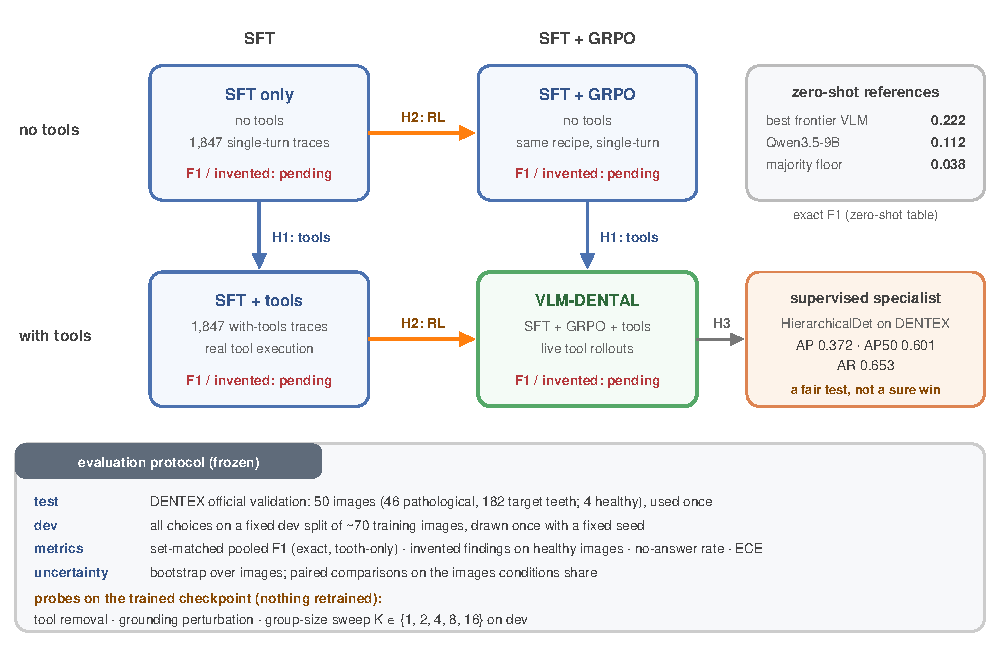
\includegraphics[width=\linewidth]{fig_design}
  \caption{Experimental design. The four conditions form a $2\times2$ (SFT vs.\ SFT$+$GRPO, with
  vs.\ without tools) trained with one recipe, so H1 (tools help) compares rows within a column
  and H2 (RL helps) compares columns within a row; H3 positions the full system against a
  supervised specialist, next to the zero-shot references of \cref{tab:zeroshot}. Result cells
  are pending the first hardware run, as in \cref{tab:main}; the protocol is frozen
  (\cref{sec:eval}).}
  \label{fig:design}
\end{figure}

\subsection{Zero-shot baselines: the case for looking again}
\label{sec:baselines}

\begin{table}[tbp]
  \centering
  \small
  \caption{Zero-shot frontier VLMs on the DENTEX validation set ($N=50$ panoramic radiographs;
  set-level matching over all annotated findings). Exact match requires the right tooth
  \emph{and} diagnosis. ECE = expected calibration error.}
  \label{tab:zeroshot}
  \begin{tabular}{lrrrrrr}
    \toprule
    Model & $N$ & FDI acc. & Exact acc. & Exact F1 & 95\% CI & ECE \\
    \midrule
    Moonshot Kimi-k3 & 50 & 64.0\% & \textbf{46.0\%} & \textbf{0.222} & [32.0, 60.0] & \textbf{0.214} \\
    Meta Llama 3.2 90B & 46 & 45.7\% & 37.0\% & 0.098 & [23.9, 52.2] & 0.395 \\
    Gemini 3.5 Flash & 50 & 62.0\% & 36.0\% & 0.188 & [22.0, 50.0] & 0.560 \\
    MiniMax M3 & 50 & 62.0\% & 32.0\% & 0.110 & [20.0, 44.0] & 0.493 \\
    Gemini 3.5 Flash Lite & 50 & 54.0\% & 32.0\% & 0.166 & [18.0, 46.0] & 0.596 \\
    Qwen3.5-9B (our backbone) & 49 & 53.1\% & 30.6\% & 0.112 & [18.4, 42.9] & 0.600 \\
    Majority-class floor & 50 & 38.0\% & 8.0\% & 0.038 & [2.0, 16.0] & -- \\
    Meta Llama 3.2 11B & 50 & 26.0\% & 4.0\% & 0.010 & [0.0, 10.0] & 0.678 \\
    \bottomrule
  \end{tabular}
\end{table}

\cref{tab:zeroshot} establishes the problem the agent architecture addresses. Even the best
frontier model misses more than half of the exact findings; the best-calibrated model still
carries ECE 0.21 while most models report 0.85--0.95 confidence on hallucinated positions; and a
dense 11B generalist falls \emph{below the majority-class floor}, a statistical collapse rather
than a graceful degradation. The failure modes are structural, not stochastic: quadrant
inversions from the OPG's left/right display convention, a resolution bottleneck that reduces an
early caries to a sub-patch blur, tissue-masking of periapical radiolucencies, and severe
overconfidence. Each of these maps onto a specific tool in \cref{tab:tools} --- which is the
design rationale of the suite, not a post hoc story: grounding corrects spatial disorientation,
\texttt{zoom\_crop} bypasses the resolution bottleneck, \texttt{window\_level} and
\texttt{enhance\_contrast} counter tissue masking, and \texttt{contralateral\_compare} tests
symmetry hypotheses before commitment.

\subsection{Main results}
\label{sec:mainresults}

\begin{table}[tbp]
  \centering
  \small
  \caption{Main results on the DENTEX validation set (pooled finding-level, set-matched);
  ``Best zero-shot frontier'' is the best row of \cref{tab:zeroshot}. Cells marked
  \todo{} are pending the first hardware training run; the experimental design and
  metric definitions are final and frozen (\cref{sec:eval}).}
  \label{tab:main}
  \footnotesize
  \setlength{\tabcolsep}{4pt}
  \begin{tabular}{@{}llccc@{}}
    \toprule
    Condition & Tools & Exact F1 $\uparrow$ & Tooth-only F1 $\uparrow$ & Invented$\downarrow$ \\
    \midrule
    Best zero-shot frontier & -- & 0.222 & -- & -- \\
    Zero-shot Qwen3.5-9B & -- & 0.112 & -- & -- \\
    Majority-class floor & -- & 0.038 & -- & -- \\
    SFT only (no tools) & -- & \todo{pending} & \todo{pending} & \todo{pending} \\
    SFT + tools & \checkmark & \todo{pending} & \todo{pending} & \todo{pending} \\
    SFT + GRPO (no tools) & -- & \todo{pending} & \todo{pending} & \todo{pending} \\
    \sys{} (SFT + GRPO) & \checkmark & \todo{pending} & \todo{pending} & \todo{pending} \\
    \midrule
    \multicolumn{5}{@{}l@{}}{Supervised specialist (HierarchicalDet), DENTEX: AP 0.372 / AP$_{50}$
    0.601 / AR 0.653 \citep{hamamci2024dentex}} \\
    \bottomrule
  \end{tabular}
\end{table}

\cref{tab:main} is the paper's primary claim table: does the agentic recipe beat zero-shot
inference and the same backbone without tools (H1: tools help; H2: RL helps), and where does it
stand against a supervised specialist (H3, framed as a fair test rather than a guaranteed win).
The training runs are in progress; all result cells are filled from the frozen evaluation
protocol above as runs complete.

\subsection{Mechanism analysis: does tiered perturbation elicit self-correction?}
\label{sec:mechanism}

Before any training, the corpus itself tests the central design claim of \cref{sec:perturbation}:
did the perturbation hook make the \emph{teacher} --- an expert-level frontier model with no
verbal hints --- actually inspect, judge, and correct grounding output, rather than scriptedly
nudge? We answer this by re-walking every with-tools trace (8{,}404 analysed
\texttt{locate\_tooth} returns) and reconstructing, for each located tooth, the box the teacher
was shown, the reference box, and every subsequent \texttt{nudge\_crop} applied to that box
through the trace. The shown box is recovered from the retained observation payloads (exact
post-perturbation boxes; validated at zero mean coordinate error against reference boxes on the
clean tier) or, where context truncation removed the observation, from the teacher's own
downstream \texttt{bbox} arguments, attributed by nearest center. Each attributed nudge is then
classified by direction: \emph{corrective} if its shift moved the working box toward the
reference center (cosine $>0.3$), \emph{away} if against it, \emph{rescaling} otherwise.

\begin{table}[tbp]
  \centering
  \small
  \caption{Correction behavior by perturbation tier, over the ground-truth-anchored subset of
  locate returns (reference box $=$ expert box; pathology cohorts). P(nudge) counts any
  attributed \texttt{nudge\_crop}; P(corrective) counts locates with at least one
  corrective-direction nudge; IoU after is over corrected locates. The clean tier is a control:
  with a correct box, corrective nudges are rare.}
  \label{tab:nudgetier}
  \begin{tabular}{lrrrrrr}
\toprule
Tier & $n$ & P(nudge) & P(corrective) & IoU before & IoU after & $\Delta$IoU \\
\midrule
none & 2,338 & 19.4\% & 1.1\% & 1.00 & 0.27 $\pm$ 0.18 & -0.73 \\
small & 1,337 & 23.1\% & 13.6\% & 0.45 & 0.45 $\pm$ 0.18 & -0.01 \\
big & 1,493 & 47.2\% & 38.4\% & 0.10 & 0.24 $\pm$ 0.18 & +0.15 \\
\bottomrule
\end{tabular}
\end{table}

\begin{figure}[tbp]
  \centering
  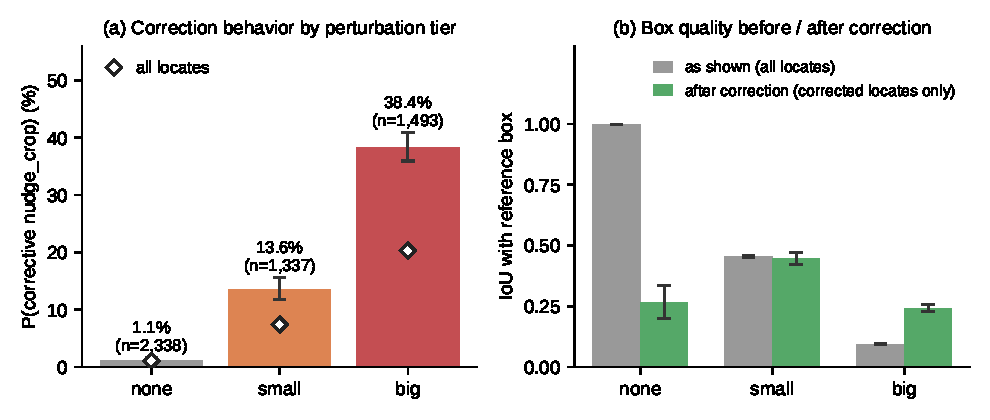
\includegraphics[width=\linewidth]{fig_nudge_tier}
  \caption{(a) Corrective \texttt{nudge\_crop} usage rises monotonically with perturbation
  severity on the ground-truth-anchored subset (bars, with Wilson 95\% intervals; the rates of
  \cref{tab:nudgetier}); diamonds give the same rate over all locate returns, including
  detector-anchored ones. (b) Mean IoU with the reference box as shown (over all locates with a
  recovered shown box) and after correction (over corrected locates only), with 95\% intervals
  of the mean; the two bars average different sets of locates, so their difference is not a
  paired gain. The ``none'' after-bar reflects the few corrective nudges on clean boxes
  (1.1\% of that tier), which are mostly reframing rescales rather than corrections.}
  \label{fig:nudgetier}
\end{figure}

\cref{tab:nudgetier} and \cref{fig:nudgetier} show the intended gradient, cleanly and
monotonically: corrective nudges on 38.4\% of large offsets, 13.6\% of small ones, and 1.1\% of
clean boxes. The clean-tier control matters: the teacher does not nudge reflexively --- with a
correct box it proceeds 98.9\% of the time, so the gradient is driven by the \emph{observed}
displacement, not a scripted habit. The small tier behaves exactly as designed as a judgment
call: nudges there are frequent (23.1\%) but only sometimes corrective (13.6\%), consistent with
the zoom margin often absorbing a small offset. On corrected large offsets, mean IoU against the
expert box improves from 0.095 to 0.243 per correction episode --- partial on average, because a
single nudge rarely lands perfectly --- with individual recoveries as large as IoU 0.066
$\to$ 0.938 on a DENTEX training image (\cref{fig:concept}; further episodes in \cref{fig:gallery}). The residual gap is not silently
absorbed: uncorrected spatial drifts are exactly what the verifier's third rejection category
(11 traces) caught and repaired during corpus construction.

Two further observations sharpen the picture. First, the split by reference type (full split in
\cref{app:mechanism}): on
\emph{detector-anchored} locates (exploratory calls during healthy-scan full-arch surveys, where
the reference is the detector's own box), correction is much rarer (5.0\% on large offsets vs.\
38.4\% ground-truth-anchored) --- during rapid systematic surveys the teacher surveys broadly
and does not inspect each exploratory box as carefully. We report this honestly; the
demonstrated skill this paper targets is the ground-truth-anchored pathology workflow. Second,
nudge \emph{rescales} skew small (scale $<1$): the dominant corrective pattern is
tighten-after-shift, matching radiologist behavior of zooming into a suspected lesion after
centering it.

\begin{figure}[!tb]
  \centering
  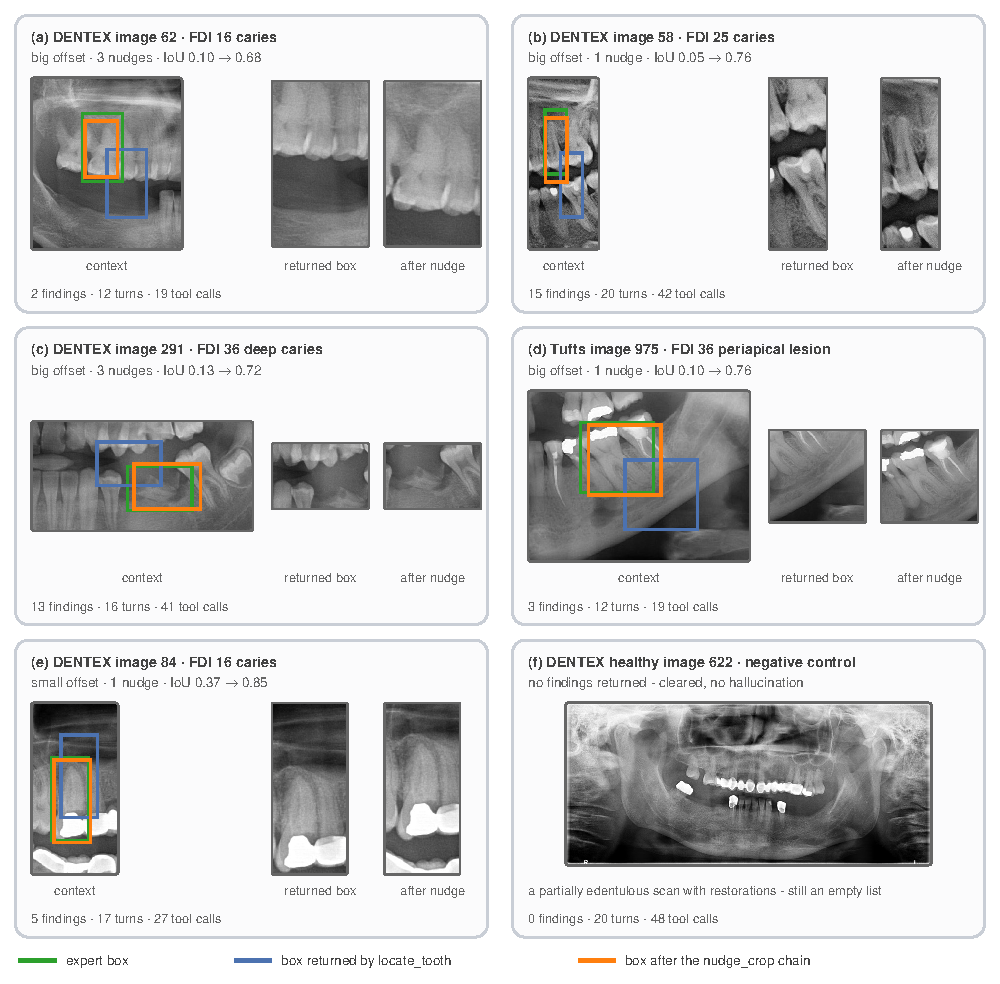
\includegraphics[width=\linewidth]{fig_gallery}
  \caption{Six verified with-tools episodes from the released corpus (five pathology, one healthy
  negative control), from two institutions. Each pathology panel shows the episode in context
  (expert box green, box returned by \texttt{locate\_tooth} blue, box after the
  \texttt{nudge\_crop} chain orange) and the crops the policy inspected before and after
  correcting; the header gives the offset tier, the number of nudges, and the IoU with the
  full-tooth expert box. (a) A three-nudge inspect--correct--re-inspect loop; (b) one nudge among
  15 findings and 42 tool calls; (c) a deep-caries tooth with a three-step chain; (d) a Tufts
  periapical lesion; (e) a small-offset judgment call; (f) a healthy scan cleared without a
  hallucinated finding. Tiers are recovered geometrically from the returned box (the
  perturbation metadata is stripped at release), and a policy that also rescales to focus can show a
  lower IoU than the displacement it recovered.}
  \label{fig:gallery}
\end{figure}

\subsection{Ablations and robustness checks}
\label{sec:ablations}

All ablation machinery is implemented and runs on a trained checkpoint with nothing retrained;
results are reported here as the runs complete.

\paragraph{Tool-removal probe.}
A tool is removed from the registry (absent from the prompt's tool list; calls to it return the
standard ``not recognized'' error), and we record both the score drop and how often the trained
agent attempts the missing tool. This measures dependence on each tool, including
\texttt{nudge\_crop}; because the checkpoint was trained with the tools present, it is a
dependence probe, not the score of a tool-free model --- the no-tools training arms in
\cref{tab:main} serve the latter role. \todo{pending}

\paragraph{Grounding-perturbation probe.}
Every \texttt{locate\_tooth} box at evaluation time is displaced by a fixed pseudo-random
fraction of its own size (the same wrong box for the same image and tooth across conditions, so
comparisons stay paired), and we report the IoU of the agent's working box against the annotated
tooth before and after its last \texttt{nudge\_crop}, plus how much of the annotated tooth the
last \texttt{zoom\_crop} actually shows. This is a stress test of the trained policy's
self-correction --- the deployed version of \cref{sec:mechanism}. \todo{pending}

\paragraph{Group-size sweep.}
GRPO group sizes $K \in \{1, 2, 4, 8, 16\}$ on the dev split, reporting pooled F1 per K with
paired comparisons and training cost; reports, never selects. \todo{pending}

% ---------------------------------------------------------------------------
\section{Limitations}
\label{sec:limitations}

\paragraph{No prospective clinician study.}
Our validity anchor is DENTEX's dentist-verified ground truth (each image was annotated by a
final-year dental student and verified by an expert dentist with over 15 years of experience),
together with automated checks of reasoning grounding by a cross-family LLM judge. This
validates against expert labels, not against a prospective, blinded review by practicing
clinicians on new cases. A reader study is the natural next step.

\paragraph{Pending trained-policy results.}
The training-side evaluations (SFT, GRPO, and ablations on the trained agent) are designed,
frozen, and implemented, but the runs are not complete. Those cells are marked as pending
instead of extrapolated. The completed evidence (zero-shot baselines, grounding-tool
validation, and the corpus-level mechanism analysis) stands independently, but end-to-end
claims cannot be made until the runs are complete.

\paragraph{Synthetic perturbations are not real detector errors.}
The tiered perturbation draws offsets from fixed configured ranges, not from the grounding
model's actual error distribution. This keeps demonstrations stable as the detector improves
(\cref{sec:perturbation}), but the training distribution of box errors is synthetic: uniform
random offsets with random signs, unlike the structured errors a real detector makes (for
example adjacent-tooth confusions and root-tip truncations). The evaluation-time
grounding-perturbation probe (\cref{sec:ablations}) measures robustness to a related synthetic
distribution. Robustness to the detector's true error modes is best assessed by swapping in
improved detector weights, which our decoupling makes safe for the trace corpus but which does
not replace measuring it.

\paragraph{Demonstrated vs.\ learned correction.}
\cref{sec:mechanism} measures the \emph{teacher's} behavior in the demonstrations, which is the
skill the student is trained to acquire, not the trained policy's behavior at inference. The
policy-side version of the same analysis is the grounding-perturbation probe, which awaits the
trained checkpoint. Demonstrated behavior is necessary but not sufficient for learned behavior.

\paragraph{Scale and scope.}
The corpus holds 3{,}694 traces over two institutions and four DENTEX diagnosis classes (plus
Tufts' four-class taxonomy). Prior work suggests that a few hundred verified examples can
suffice for medical RL fine-tuning \citep{hu2025medvlmr1}, but the corpus is modest in size and
the DENTEX test set contains only 50 images, so confidence intervals on it are wide; we report
them rather than over-reading point estimates. The tool suite covers radiologist-like
inspection primitives. Measurement and calibration tools (lesion sizing, periodontal probing
analogues) and anomaly detection beyond the four classes are out of scope.

\paragraph{Automated verification is not expert review.}
The verifier is a frontier model from a different family than the generator, audited against
expert labels, and its rejection taxonomy shows that it catches real failures. Automated
verification nevertheless has blind spots that human clinical review would not. We mitigate
this with cross-family verification, ground-truth anchoring of every correctness claim, and
release of the full corpus and audit trail so that others can re-audit it.

\paragraph{Harness and serving evidence.}
The rules-only condition is a prompt-identity control, not a proposed source of diagnostic
improvement. Skills add procedural context and may help or distract, so their effects require
paired dev-split measurements. A BF16 merged target is numerically different from a 4-bit
QLoRA serving target, so speed or equivalence cannot be attributed to speculation across those
targets. Multimodal and MTP support and memory feasibility must be established for the pinned
runtime and hardware; a recognized configuration flag is not evidence of a completed run.
Neither the harness nor speculative decoding establishes clinical validity.

% ---------------------------------------------------------------------------
\section{Conclusion}
\label{sec:conclusion}

We presented \sys{}, an agentic VLM for panoramic dental radiograph diagnosis built on a
principle we argue is the right contract between a reasoning policy and its tools in any domain
with learned components: \emph{grounding is a hypothesis to interrogate, not an answer to
trust}. Concretely, the policy learns to correct its grounding tool (\texttt{nudge\_crop},
box-relative and data-only), and it can only learn this because the training signal deliberately
exposes tool error: a tiered perturbation mechanism that is decoupled from the detector's real
accuracy --- so demonstrations never go stale --- and that never announces errors verbally ---
so the learned behavior survives to inference time. The same philosophy appears in the reward:
complexity-scaled efficiency that exempts exactly the locate-and-correct calls the task
genuinely needs, and a ground-truth-anchored, multi-finding accuracy term that an LLM judge
cannot be hacked into.

The completed evidence supports each design decision: zero-shot frontier VLMs fail on DENTEX
for structural reasons that map one-to-one onto the tool suite; the grounding tool is strong
enough to be useful and imperfect enough to need correcting; and the perturbation mechanism
elicits a clean, monotone correction gradient in 3{,}694 verified demonstrations (38.4\% of
large offsets corrected, 1.1\% of clean boxes) with recoveries up to IoU 0.066 $\to$ 0.938 ---
demonstrated judgment, not scripted steps. The end-to-end training results on the frozen
evaluation protocol are the immediate next step; the pipeline, corpus, audit tooling, and
protocol are released to make every number in this paper regenerable (artifact map and
regeneration commands in \cref{app:repro}).


\bibliographystyle{plainnat}
\bibliography{refs}

\appendix
% ---------------------------------------------------------------------------
\appendix

\section{Perturbation configuration}
\label{app:perturbation}

The exact configuration used for trace generation is given in \cref{tab:perturbconfig}.

\begin{table}[htbp]
  \centering
  \small
  \caption{Exact tiered-perturbation configuration used for trace generation. Offsets are drawn
  uniformly per axis with a random sign and applied with \texttt{nudge\_crop}'s own
  shift-and-clamp math, so every shown box is one the correction tool could produce or fix. The
  unperturbed box is logged internally per call (\texttt{true\_bbox}, \texttt{perturb\_tier}) and
  never shown to the model.}
  \label{tab:perturbconfig}
  \footnotesize
  \setlength{\tabcolsep}{4pt}
  \begin{tabular}{@{}lrp{3.9cm}p{4.6cm}@{}}
    \toprule
    Tier & Probability & Offset magnitude (per axis, box-relative) & Intent \\
    \midrule
    none & 0.45 & $0$ & Clean accept-and-proceed demonstration \\
    small & 0.25 & $\mathrm{U}(0.12, 0.28)$, random sign & Genuine judgment call; not resolved by the prompt \\
    big & 0.30 & $\mathrm{U}(0.45, 0.75)$, random sign & Visually self-evident without any verbal cue \\
    \bottomrule
  \end{tabular}
\end{table}

Rates are fixed constants, deliberately decoupled from the grounding detector's measured
accuracy so that improving the detector never invalidates existing demonstrations
(\cref{sec:perturbation}).

\section{Mechanism analysis: full split by reference type}
\label{app:mechanism}

\cref{tab:mechanismsplit} reports the correction-behavior analysis split by reference type;
\cref{sec:mechanism} discusses the ground-truth-anchored rows in the main text.

\begin{table}[htbp]
  \centering
  \small
  \caption{Corrective-nudge behavior split by reference type, regenerated from the released
  corpus. \emph{GT-anchored}: the locate call was ground-truth-grounded (annotated tooth;
  pathology cohorts) and the reference box is the expert box. \emph{Detector-anchored}:
  exploratory calls (dominated by healthy-scan full-arch surveys), where the reference is the
  detector's own box. During rapid surveys the teacher corrects far less often per box --- a
  real behavioral difference we report rather than average away.}
  \label{tab:mechanismsplit}
  \begin{tabular}{llrrrr}
    \toprule
    Reference & Tier & $n$ & P(nudge) & P(corrective) & IoU before $\to$ after \\
    \midrule
    GT & none & 2{,}338 & 19.4\% & 1.1\% & 1.00 $\to$ -- \\
    GT & small & 1{,}337 & 23.1\% & 13.6\% & 0.46 $\to$ 0.45 \\
    GT & big & 1{,}493 & 47.2\% & 38.4\% & 0.10 $\to$ 0.24 \\
    \midrule
    Detector & small & 1{,}472 & 2.9\% & 1.8\% & 0.37 $\to$ 0.38 \\
    Detector & big & 1{,}764 & 6.9\% & 5.0\% & 0.09 $\to$ 0.15 \\
    \bottomrule
  \end{tabular}
\end{table}

Recovery rates of the shown box (from retained observations or downstream \texttt{bbox}
arguments) were 0.97--1.00 in every cell; validation of observation-derived boxes against
reference boxes on the clean tier gave zero mean coordinate error.

\section{Grounding tool validation}
\label{app:grounding}

\cref{tab:grounding} summarizes the grounding tool's validation.

\begin{table}[htbp]
  \centering
  \small
  \caption{YOLOv8m grounding tool (32 FDI classes), 5-fold cross-validation on the combined
  DENTEX+Tufts pool (2{,}339 images, 46{,}808 boxes) and evaluation on the held-out target
  benchmark (50 images, 182 annotated targets, greedy one-to-one target matching). ``Target
  mAP50'' restricts evaluation to detections on annotated target teeth.}
  \label{tab:grounding}
  \begin{tabular}{lrrrr}
    \toprule
    Model & Target mAP50 & Target mAP50-95 & Precision & Recall@0.50 \\
    \midrule
    DENTEX-only (5-fold mean) & 0.909 & 0.638 & 0.939 & 0.818 \\
    DENTEX+Tufts (5-fold mean) & 0.926 & 0.644 & 0.963 & 0.775 \\
    Best fold (DENTEX+Tufts, fold 1) & \textbf{0.959} & \textbf{0.650} & \textbf{0.986} & 0.797 \\
    \bottomrule
  \end{tabular}
\end{table}

The precision/recall profile is the intended operating point for a grounding \emph{tool} inside
an agent loop: high precision so crops are plausible, non-perfect recall so that correction
(\cref{sec:nudge}) and re-location remain live skills rather than dead code paths.

\section{Verifier rejection taxonomy}
\label{app:verifier}

During first-pass verification the independent cross-family verifier rejected 92 of 3{,}694
traces (97.5\% first-pass pass rate), all subsequently repaired and re-verified to a 100\%
final yield:

\begin{enumerate}[leftmargin=*,itemsep=1pt,topsep=2pt]
  \item \textbf{False-positive pathology on healthy scans} --- 66 rejections (71.7\%). The
  generator hallucinated findings on disease-free scans; repaired to systematic negative surveys
  committing to \texttt{[]}.
  \item \textbf{Ground-truth contradictions and FDI errors} --- 15 rejections (16.3\%). Mismatched
  pathology classes or swapped quadrants; repaired via targeted re-prompting.
  \item \textbf{Uncorrected spatial drift} --- 11 rejections (12.0\%). The teacher diagnosed from
  a visibly displaced grounding box without a corrective \texttt{nudge\_crop}; repaired with
  spatial realignment. This category exists \emph{because} of the perturbation mechanism
  (\cref{sec:perturbation}) and is direct audit evidence that it creates genuine, checkable
  judgment pressure.
\end{enumerate}

In a separate decontamination pass, 105 traces in which the generator echoed its hidden
ground-truth directive in its reasoning were excised and regenerated under a dual gate (zero-leak
audit + verifier re-approval); the canonical corpus contains zero directive leaks and exact
1:1 parity between the with-tools and no-tools cohorts.

\section{Reproducibility}
\label{app:repro}

Every number in this paper is regenerable from released artifacts:
corpus statistics, tool-usage counts, and the mechanism analysis via
\texttt{scripts/paper/generate\_paper\_assets.py} over the released trace files (tables in
\texttt{paper/generated/}, figures in \texttt{paper/figures/}); all figures have SVG sources.
The evaluation protocol (\cref{sec:eval}) is implemented in the repository's evaluation
package; verbatim system prompts are extractable programmatically from the source
(\texttt{dental\_agent/paper/prompts.py}). Traces are hosted on the Hugging Face Hub;
model checkpoints and the grounding weights are synced to the same Hub organization.


\end{document}
